\documentclass[10pt,utf8]{beamer}

\mode<presentation> {
  \usetheme{Madrid}
  \setbeamercovered{transparent}
}

\usepackage{palatino}
\usepackage{graphicx}
\usepackage{array}
\usepackage{color}
\usepackage{subfigure}
\usepackage{colortbl}
\usepackage{amsmath}
\usepackage{hyperref}
\usepackage{listings}
\usepackage{fancyvrb}
\usepackage{pythonhighlight} % dnf install texlive-pythonhighlight
\usepackage{lmodern}

\setbeamertemplate{caption}{\raggedright\insertcaption\par} %turn off caption prefix ("Figure")

\definecolor{delim}{RGB}{20,105,176}
\definecolor{numb}{RGB}{106, 109, 32}
\definecolor{string}{rgb}{0.64,0.08,0.08}

% Define JSON language style
% Taken from https://gist.github.com/ed-cooper/1927af4ccac39b083440d436d018d253
\lstdefinelanguage{json}{
    showspaces=false,
    showtabs=false,
    breaklines=true,
    %postbreak=\raisebox{0ex}[0ex][0ex]{\ensuremath{\color{gray}\hookrightarrow\space}},
    breakatwhitespace=true,
    basicstyle=\ttfamily\footnotesize,
    upquote=true,
    morestring=[b]",
    stringstyle=\color{string},
    literate=
     *{0}{{{\color{numb}0}}}{1}
      {1}{{{\color{numb}1}}}{1}
      {2}{{{\color{numb}2}}}{1}
      {3}{{{\color{numb}3}}}{1}
      {4}{{{\color{numb}4}}}{1}
      {5}{{{\color{numb}5}}}{1}
      {6}{{{\color{numb}6}}}{1}
      {7}{{{\color{numb}7}}}{1}
      {8}{{{\color{numb}8}}}{1}
      {9}{{{\color{numb}9}}}{1}
      {\{}{{{\color{delim}{\{}}}}{1}
      {\}}{{{\color{delim}{\}}}}}{1}
      {[}{{{\color{delim}{[}}}}{1}
      {]}{{{\color{delim}{]}}}}{1},
}

\lstdefinestyle{java}{
    basicstyle          = \footnotesize\ttfamily,
    language            = java,
    numbers             = left,
    numberstyle         = \small,
    stepnumber          = 1,
    numbersep           = 5pt,
    backgroundcolor     = \color{white},
    showspaces          = false,
    showstringspaces    = false,
    showtabs            = false,
    frame               = single,
    tabsize             = 2,
    captionpos          = b,
    breaklines          = true,
    breakatwhitespace   = false,
    morestring          = [b]",
    stringstyle         = \color{blue},
    keywordstyle        = \color{magenta},
    commentstyle        = \color{gray},
    identifierstyle     = \color{black},
    moredelim           = **[is][\bfseries]{`}{`},
    moredelim           = **[is][\color{magenta}]{$}{$}, 
    fancyvrb            = true,
}


\title{Feeding ML models with the data from the databases in real-time }
\author{Vojtěch Juránek}
\institute[Red Hat]{Red Hat}
\date{June 15th 2024, DevConf, Brno}

\newenvironment{mylisting}
{\begin{list}{}{\setlength{\leftmargin}{1em}}\item\scriptsize\bfseries}
{\end{list}}

\newenvironment{mytinylisting}
{\begin{list}{}{\setlength{\leftmargin}{1em}}\item\tiny\bfseries}
{\end{list}}


\begin{document}

%\tikzstyle{every picture}+=[remember picture]
%\tikzstyle{na} = [baseline=-.5ex]

\begin{frame}
    \centering
    \huge{\textbf{Let's start with the demo!}}
    \vspace{1cm}
    \begin{figure}
        \centering
        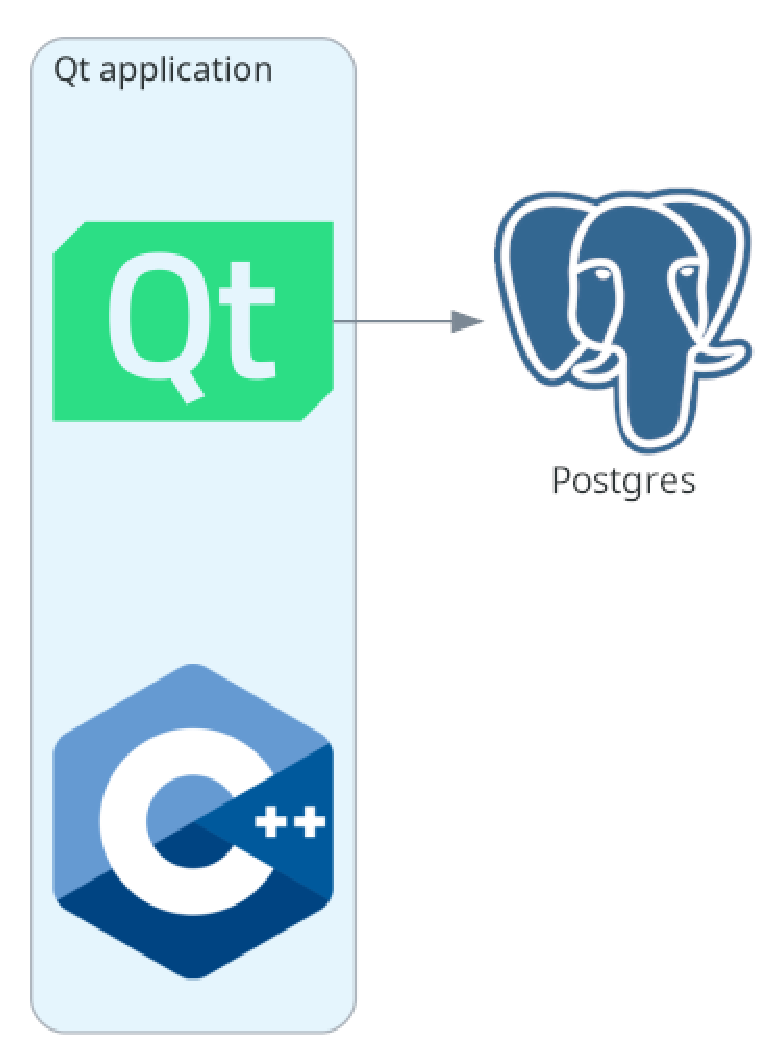
\includegraphics[height=5cm]{./img/qt_to_postgres.eps}
    \end{figure}
\end{frame}

\begin{frame}
 \titlepage
\end{frame}


\begin{frame}
    \begin{figure}
        \centering
        \includegraphics[height=8cm]{./img/mlops.eps}
        \caption{\tiny{Source: \url{https://ml-ops.org/content/end-to-end-ml-workflow}}}
    \end{figure}
\end{frame}

\begin{frame}
    \begin{figure}
        \centering
        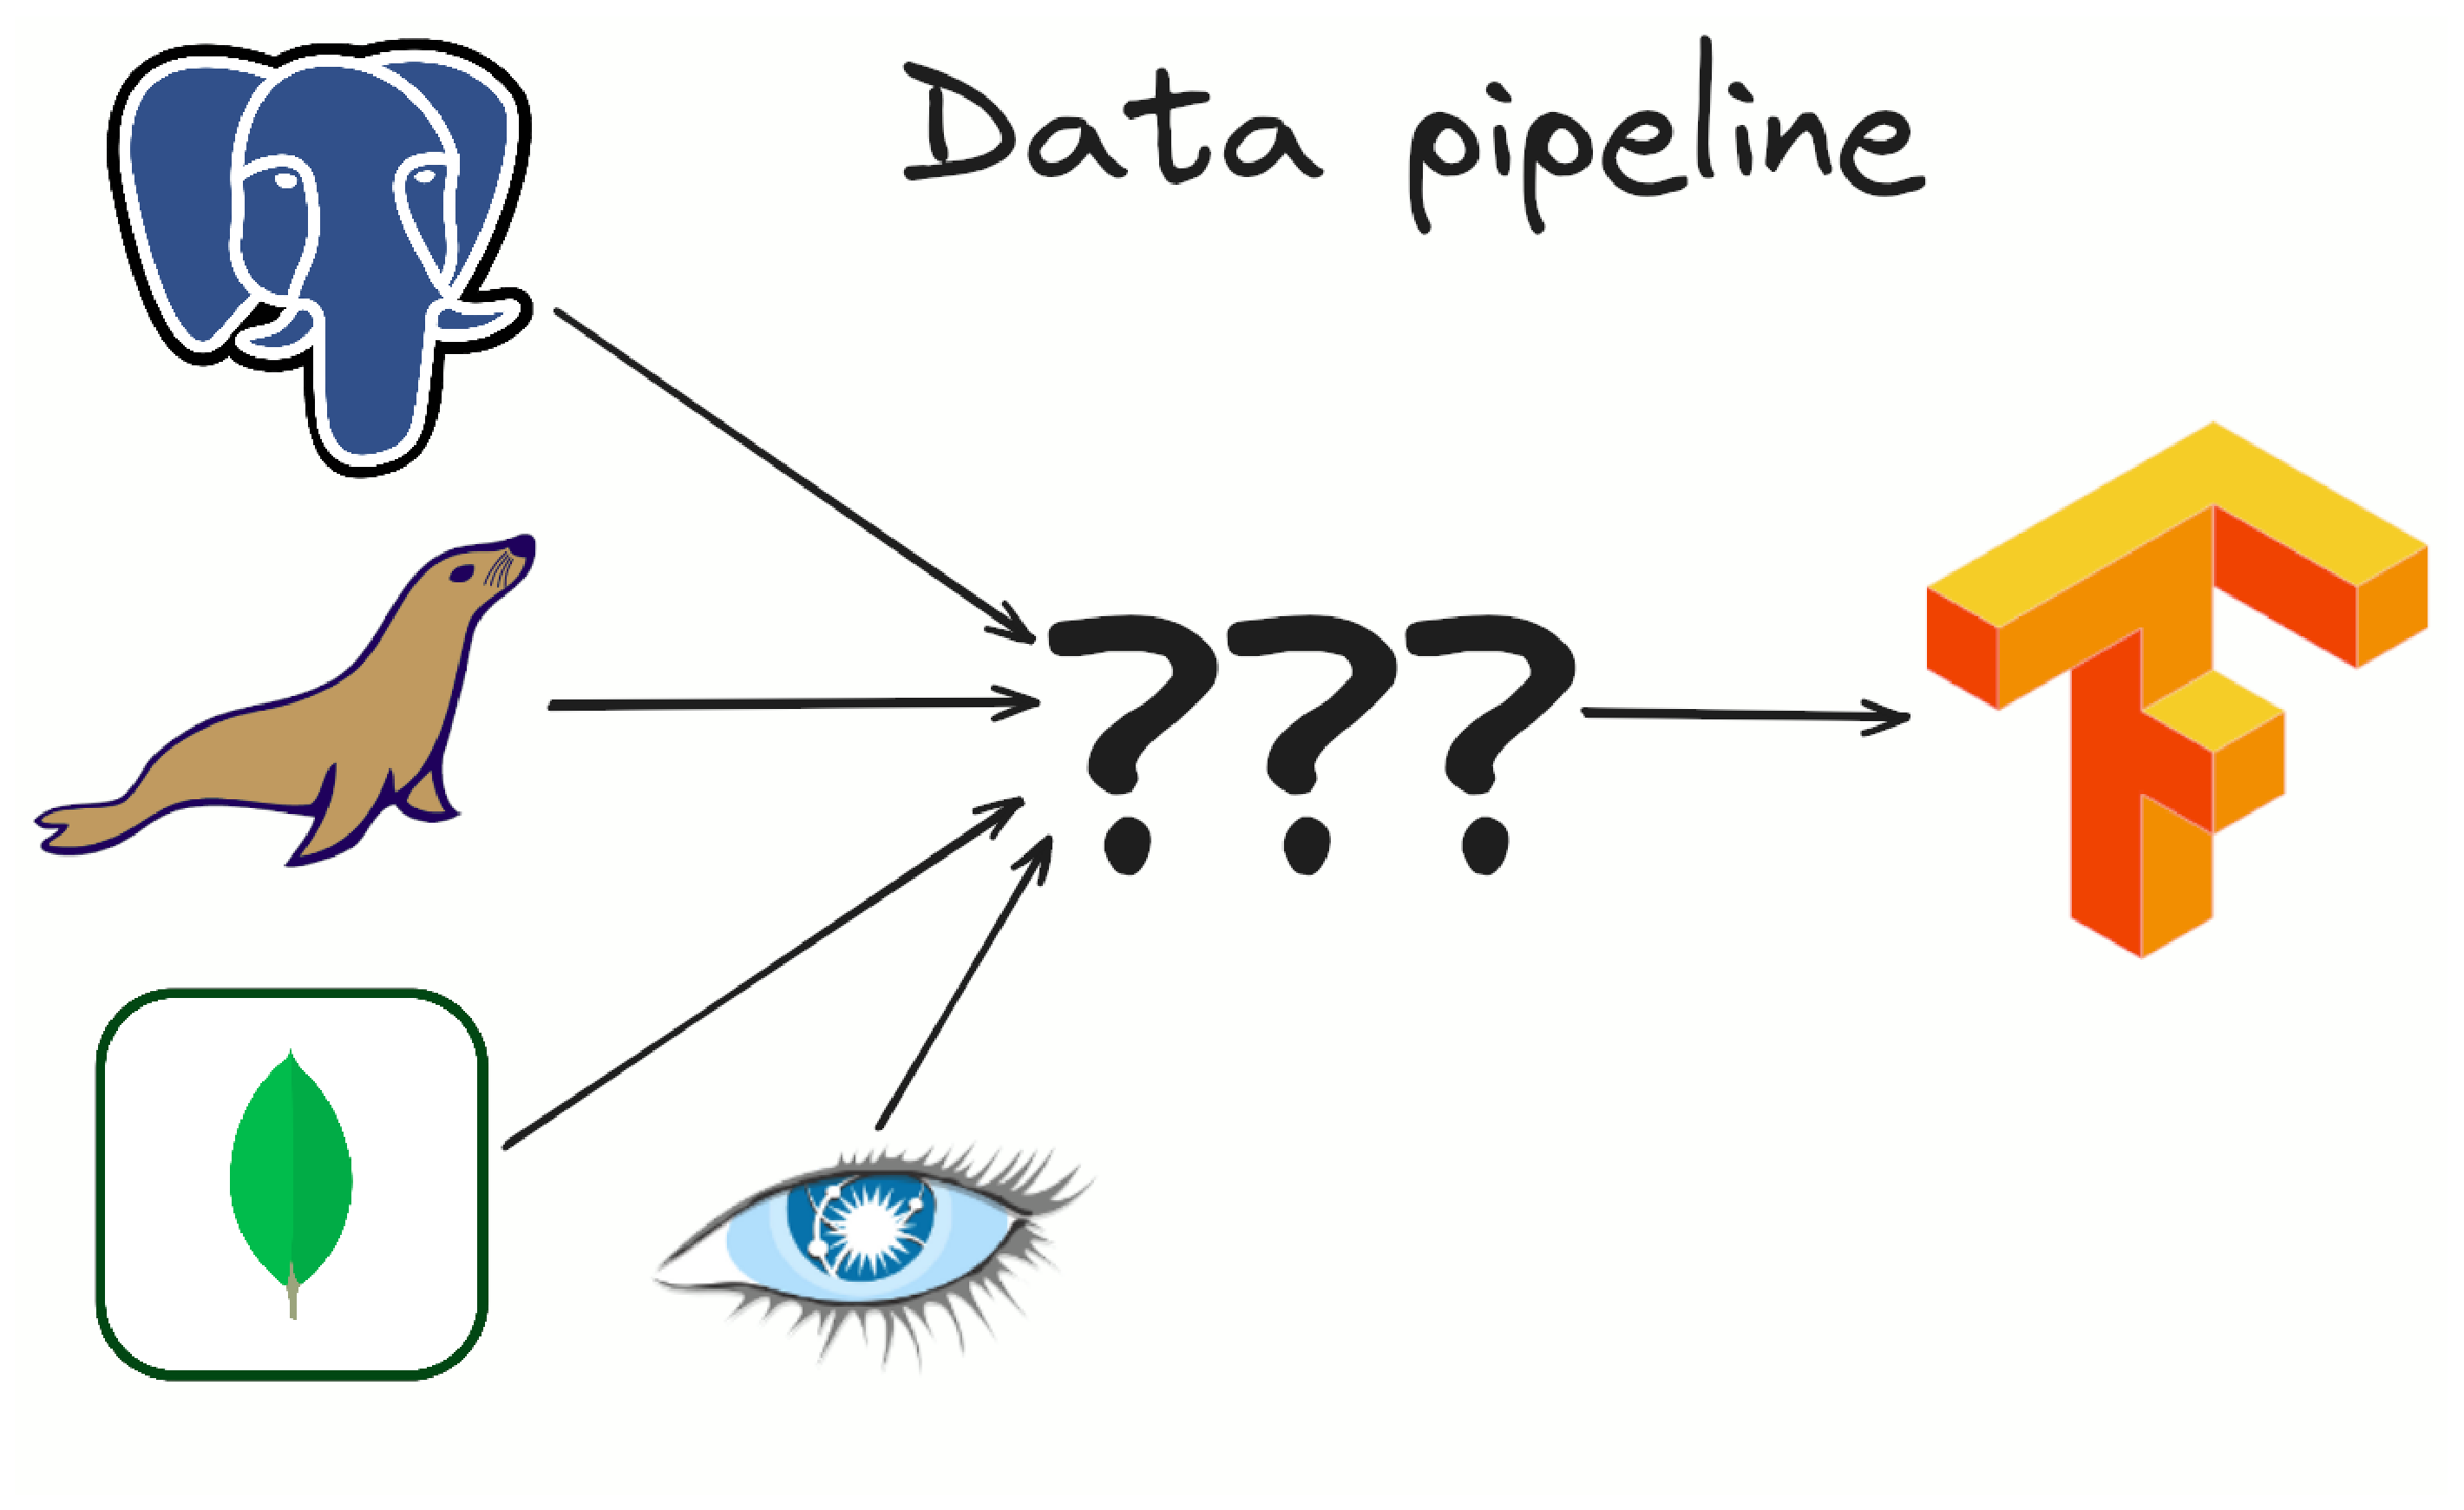
\includegraphics[height=7cm]{./img/dbs_to_tf2.eps}
    \end{figure}
\end{frame}

\begin{frame}
    \begin{figure}
        \centering
        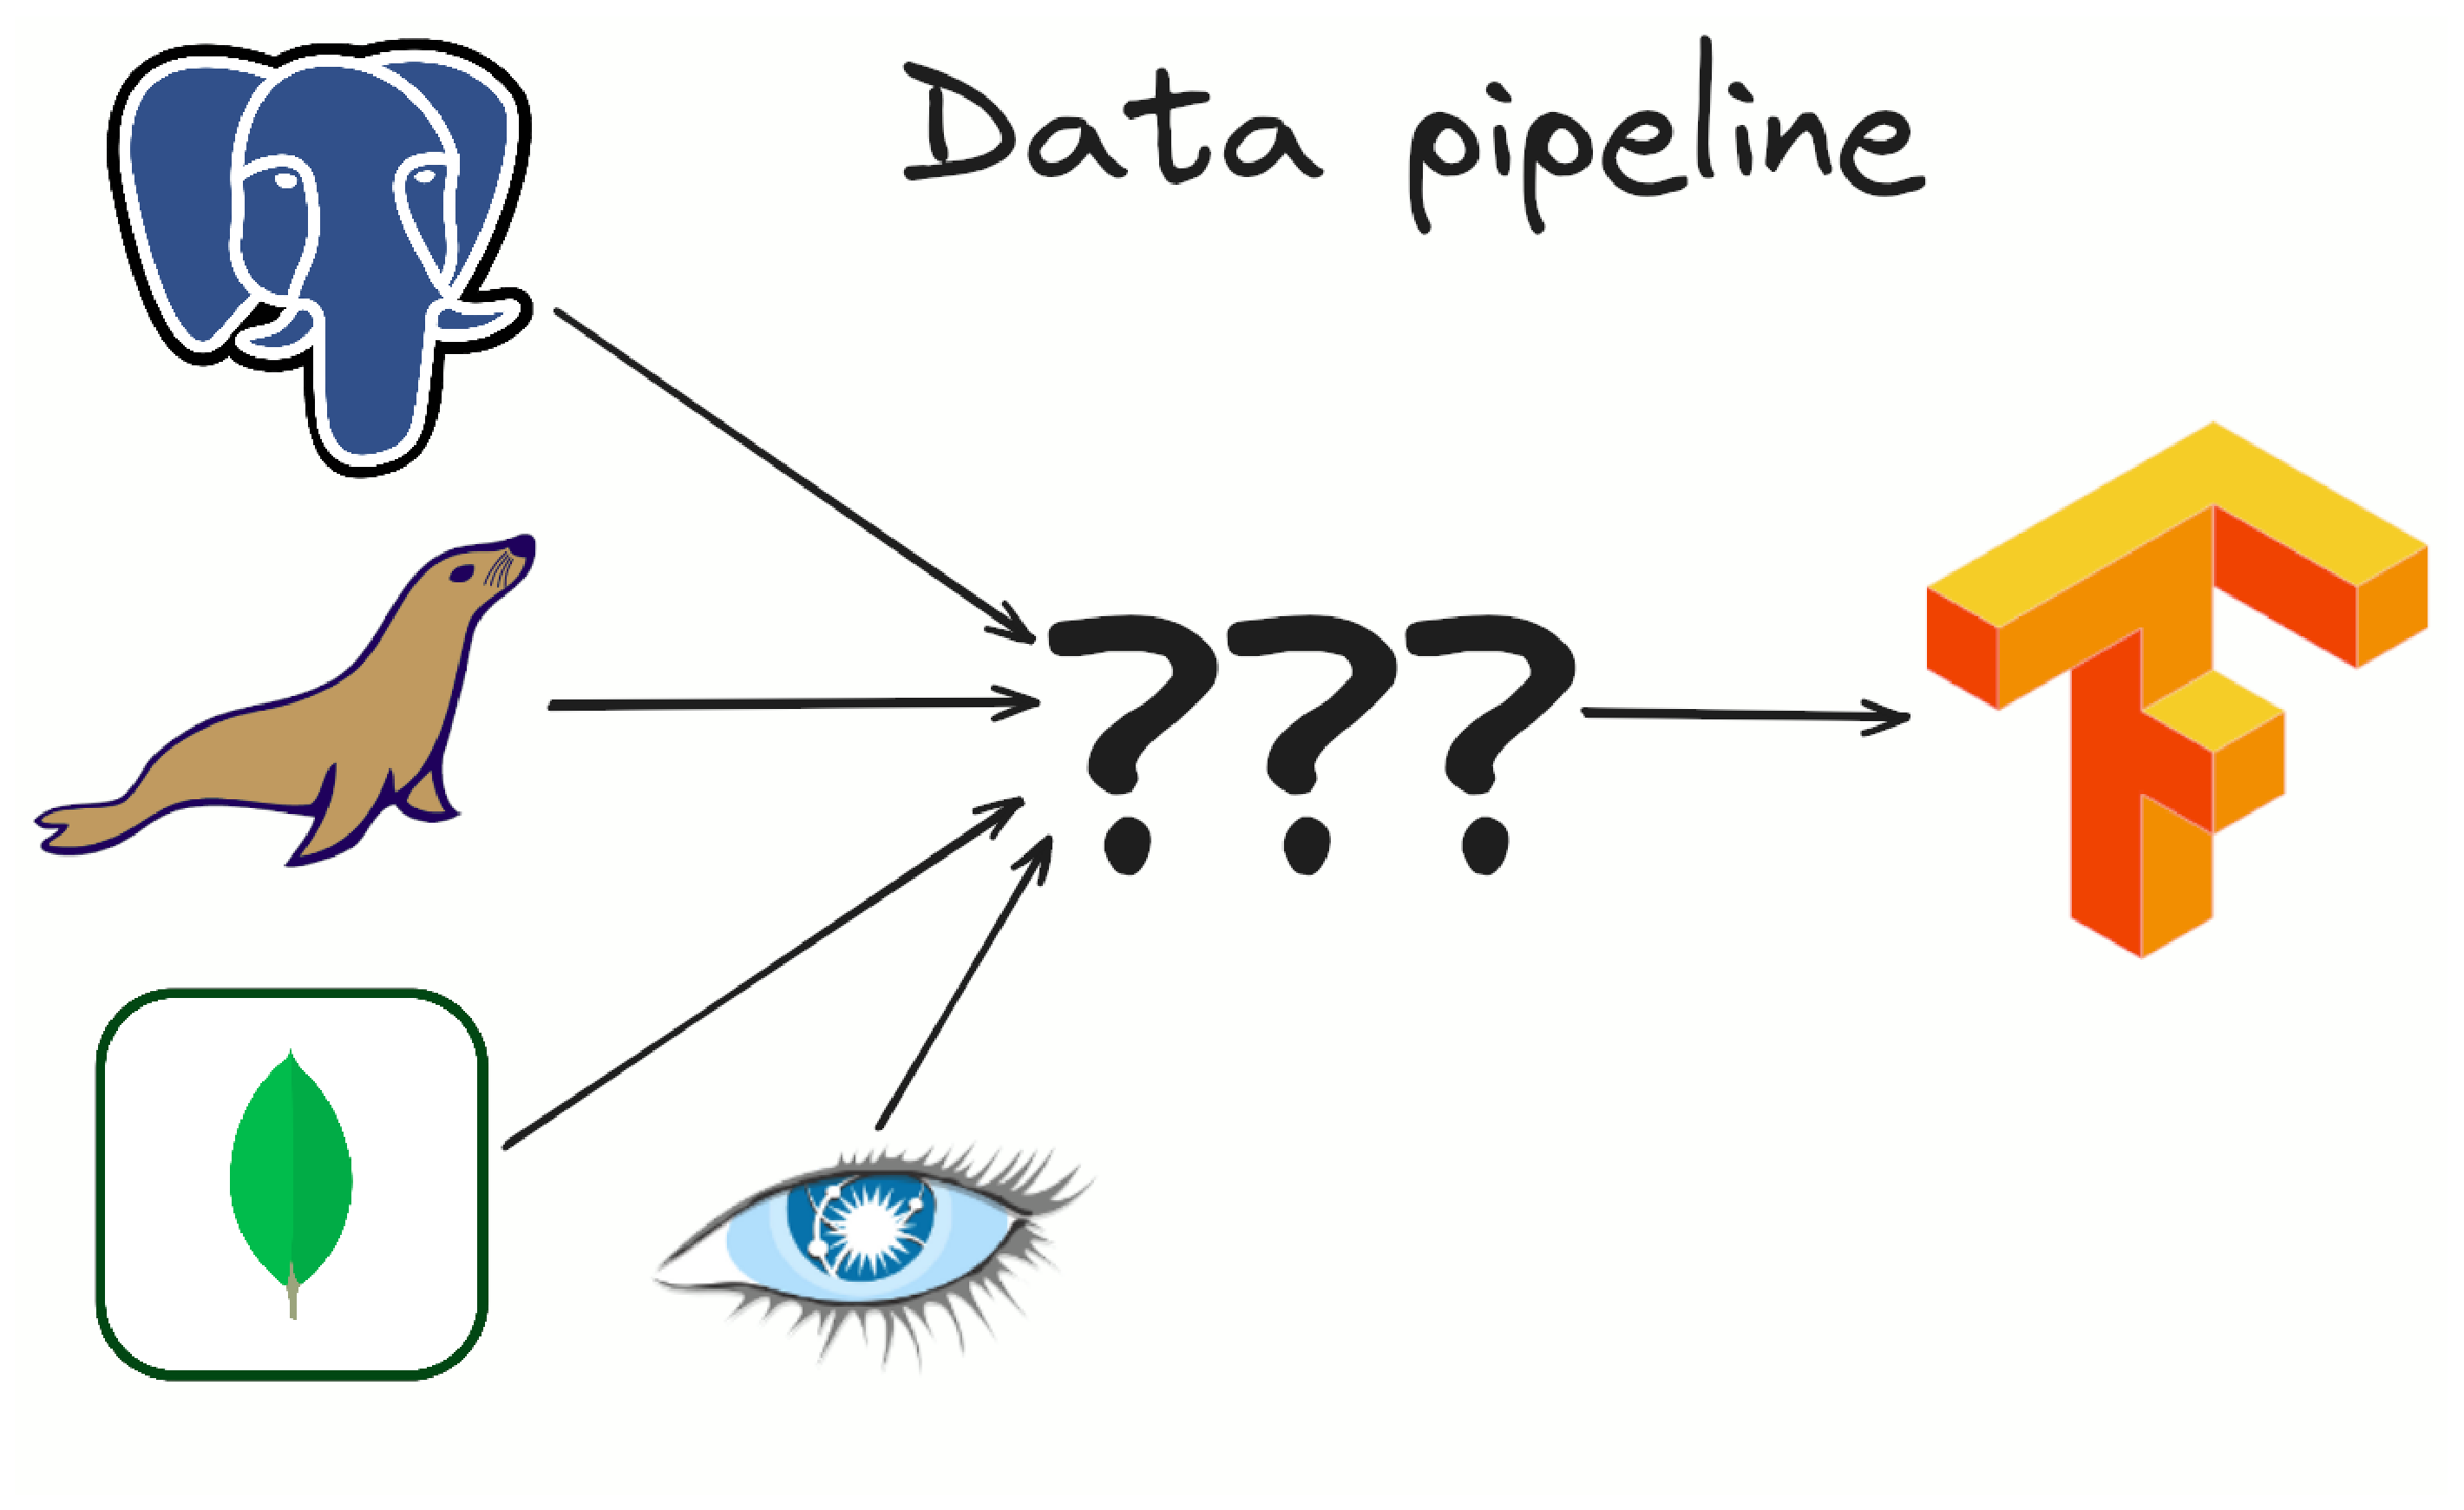
\includegraphics[height=3cm]{./img/dbs_to_tf2.eps}
    \end{figure}
    \begin{itemize}
      \item Consistent data, no data losses, no dual writes.
      \item Get all the changes without any delay in the real-time.
      \item Not overload the DB with the queries.
    \end{itemize}
\end{frame}

\begin{frame}
    \begin{figure}
        \centering
        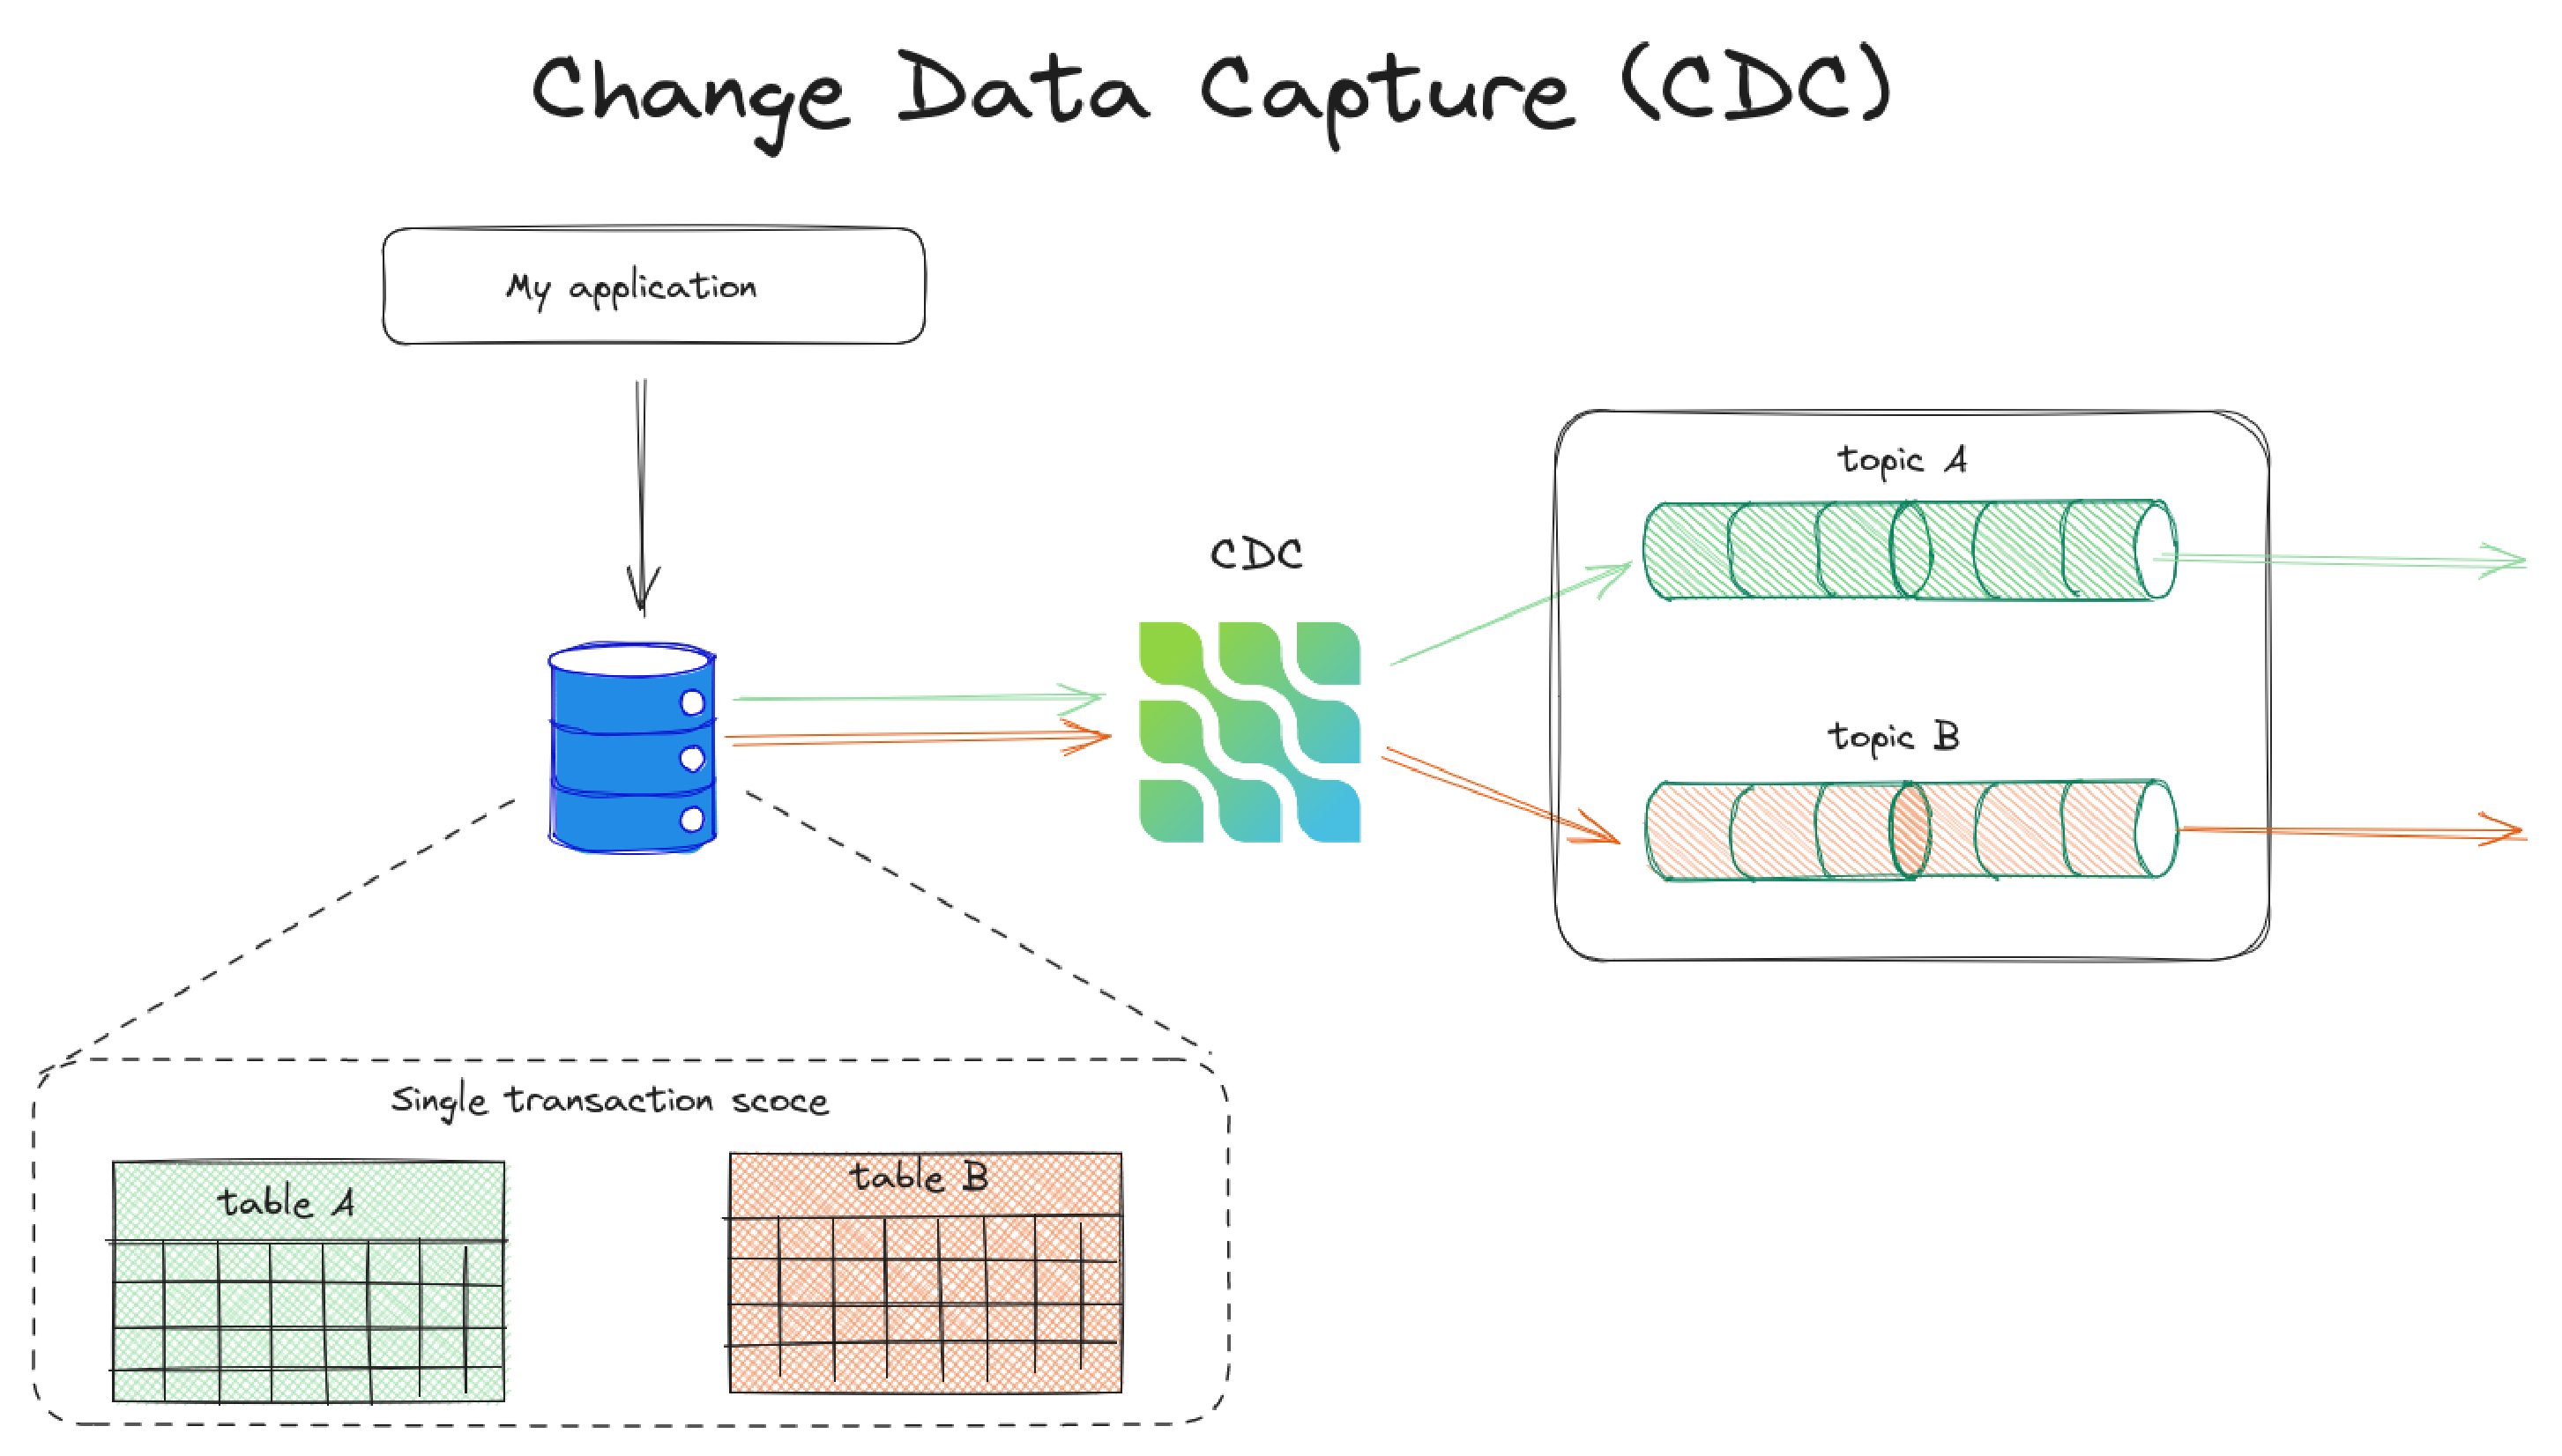
\includegraphics[height=7cm]{./img/cdc.eps}
    \end{figure}
\end{frame}

\begin{frame}
   \frametitle{Debezium}
   \begin{figure}
        \centering
        
\includegraphics[height=1.5cm]{./img/debezium.eps}
    \end{figure}
    
    \vspace{0.5cm}
    
   \begin{itemize}
     \item Leading CDC framework, de-facto industry standard.
     \item Fully open source: \textcolor{blue}{\url{https://github.com/debezium/}}
     \item Supports all major databases, including non-relational databases.
     \item Integrations with many 3rd-party tools and frameworks.
     \item Large and active user community.
     \item Used by many companies in production (see \textcolor{blue}{\href{https://debezium.io/community/users/}{Debezium public references}}).
   \end{itemize}
\end{frame}


\begin{frame}
    \begin{figure}
        \centering
        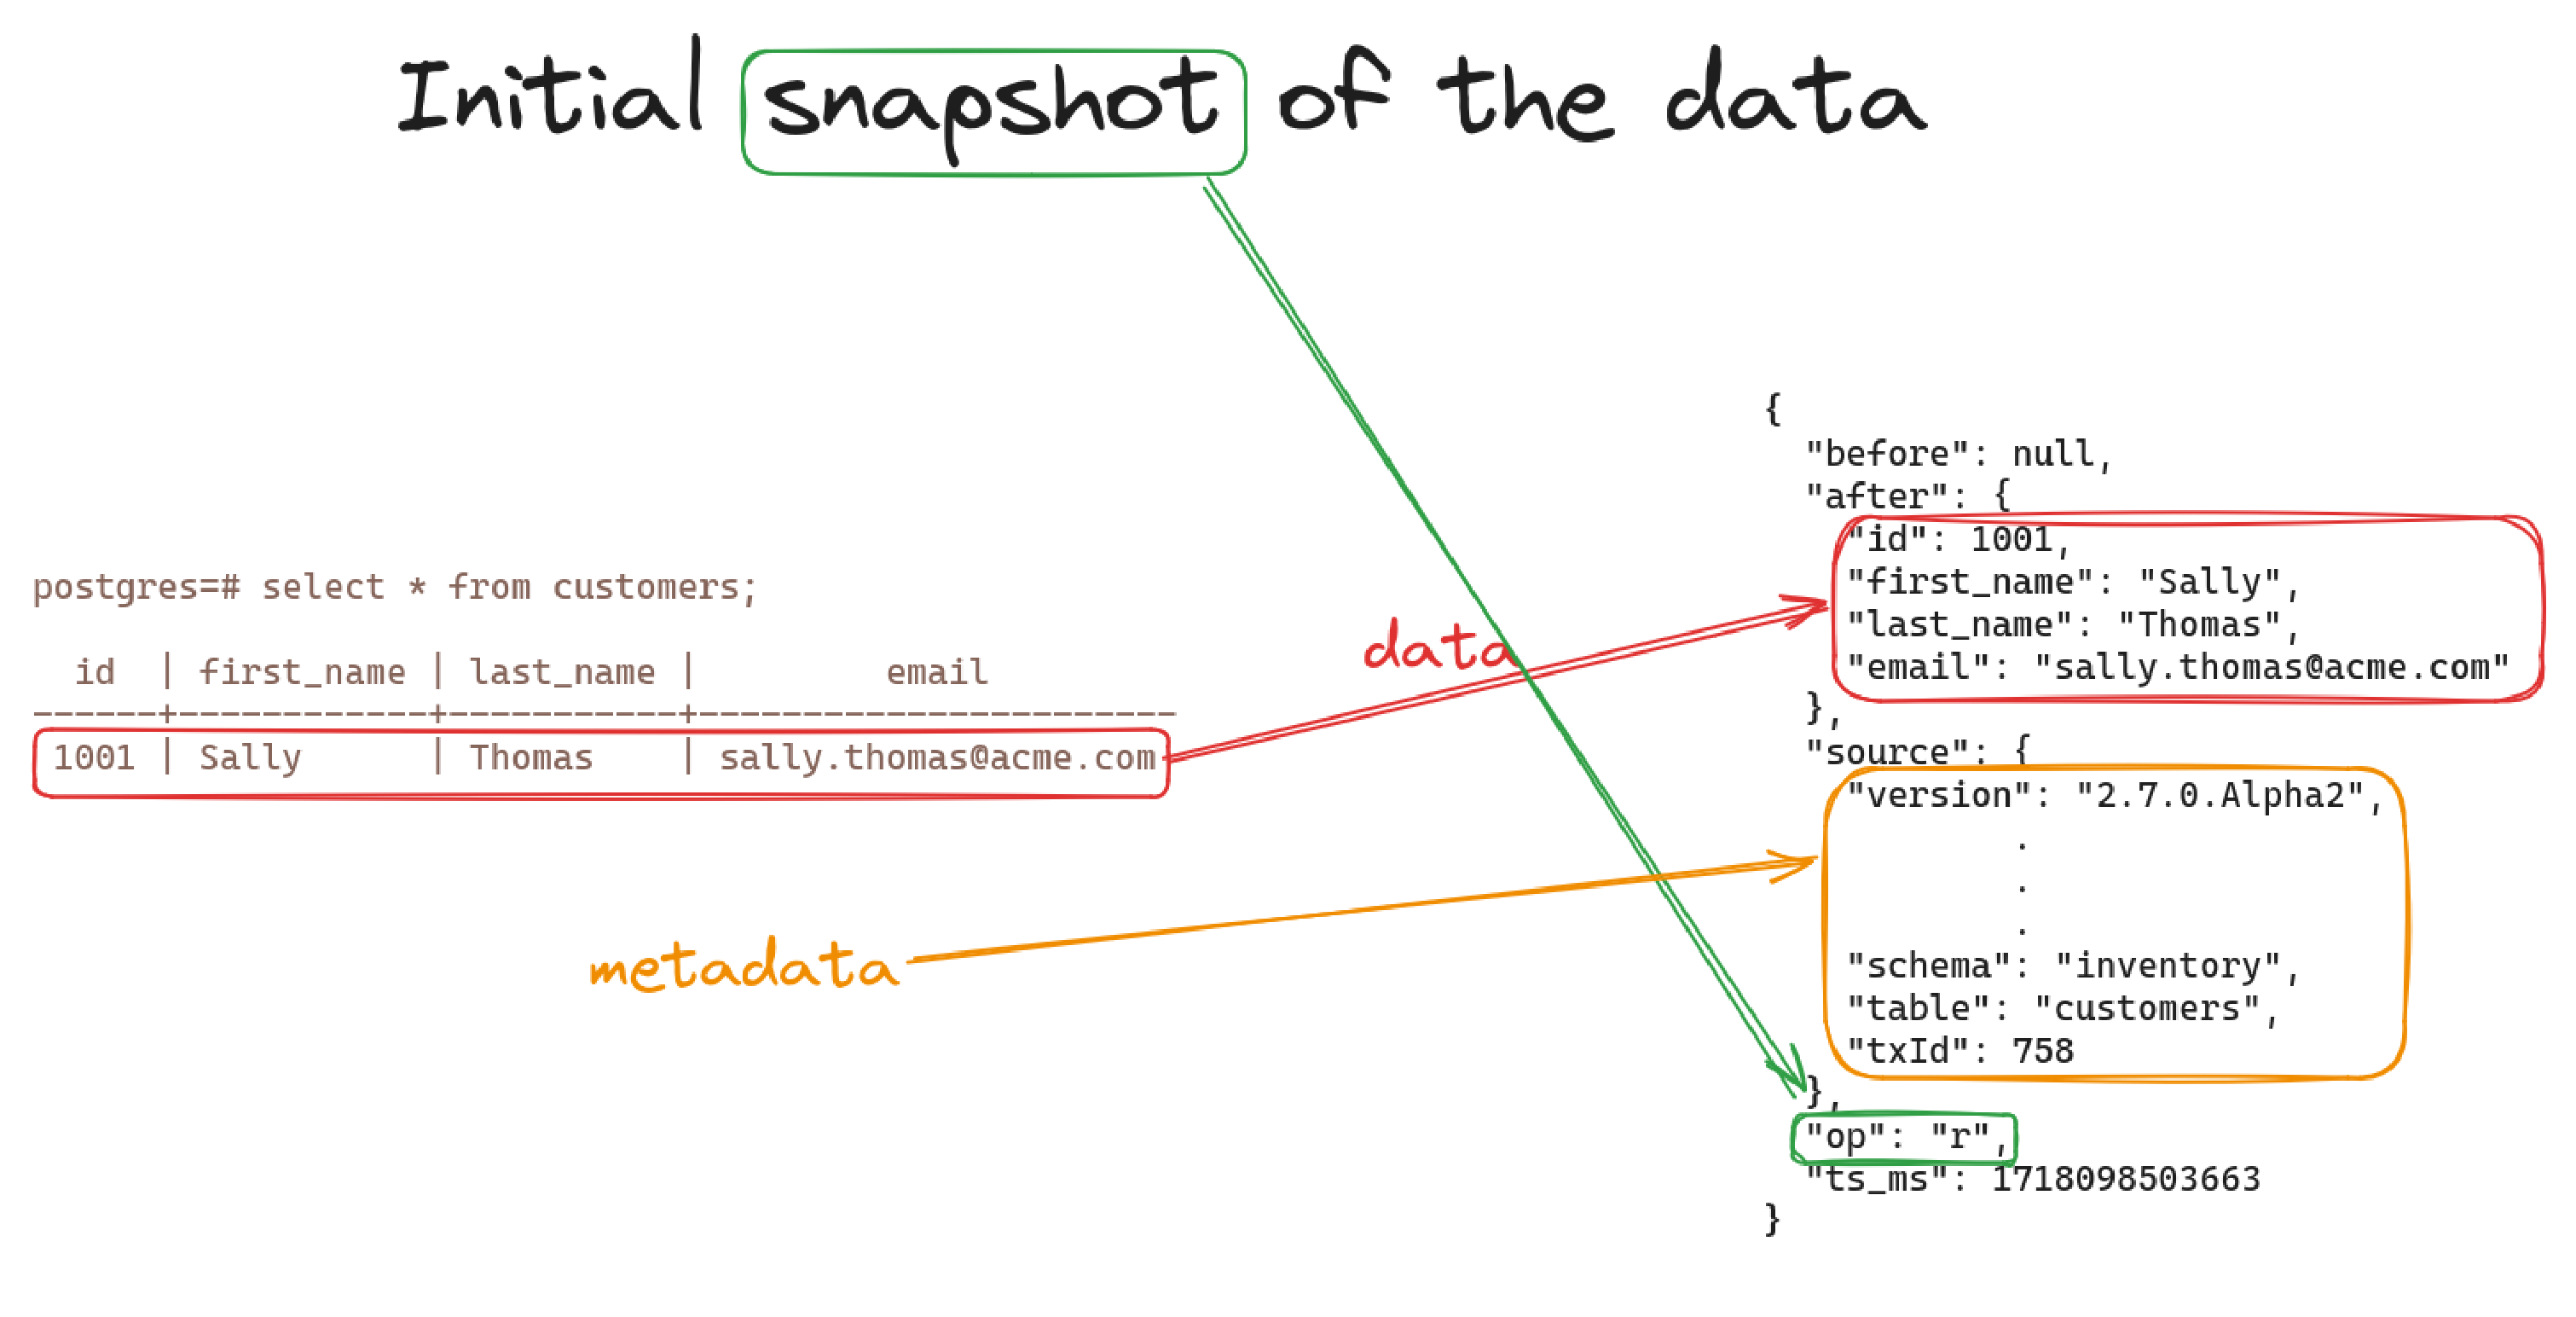
\includegraphics[height=6cm]{./img/initial_snapshot_data.eps}
    \end{figure}
\end{frame}

\begin{frame}
    \begin{figure}
        \centering
        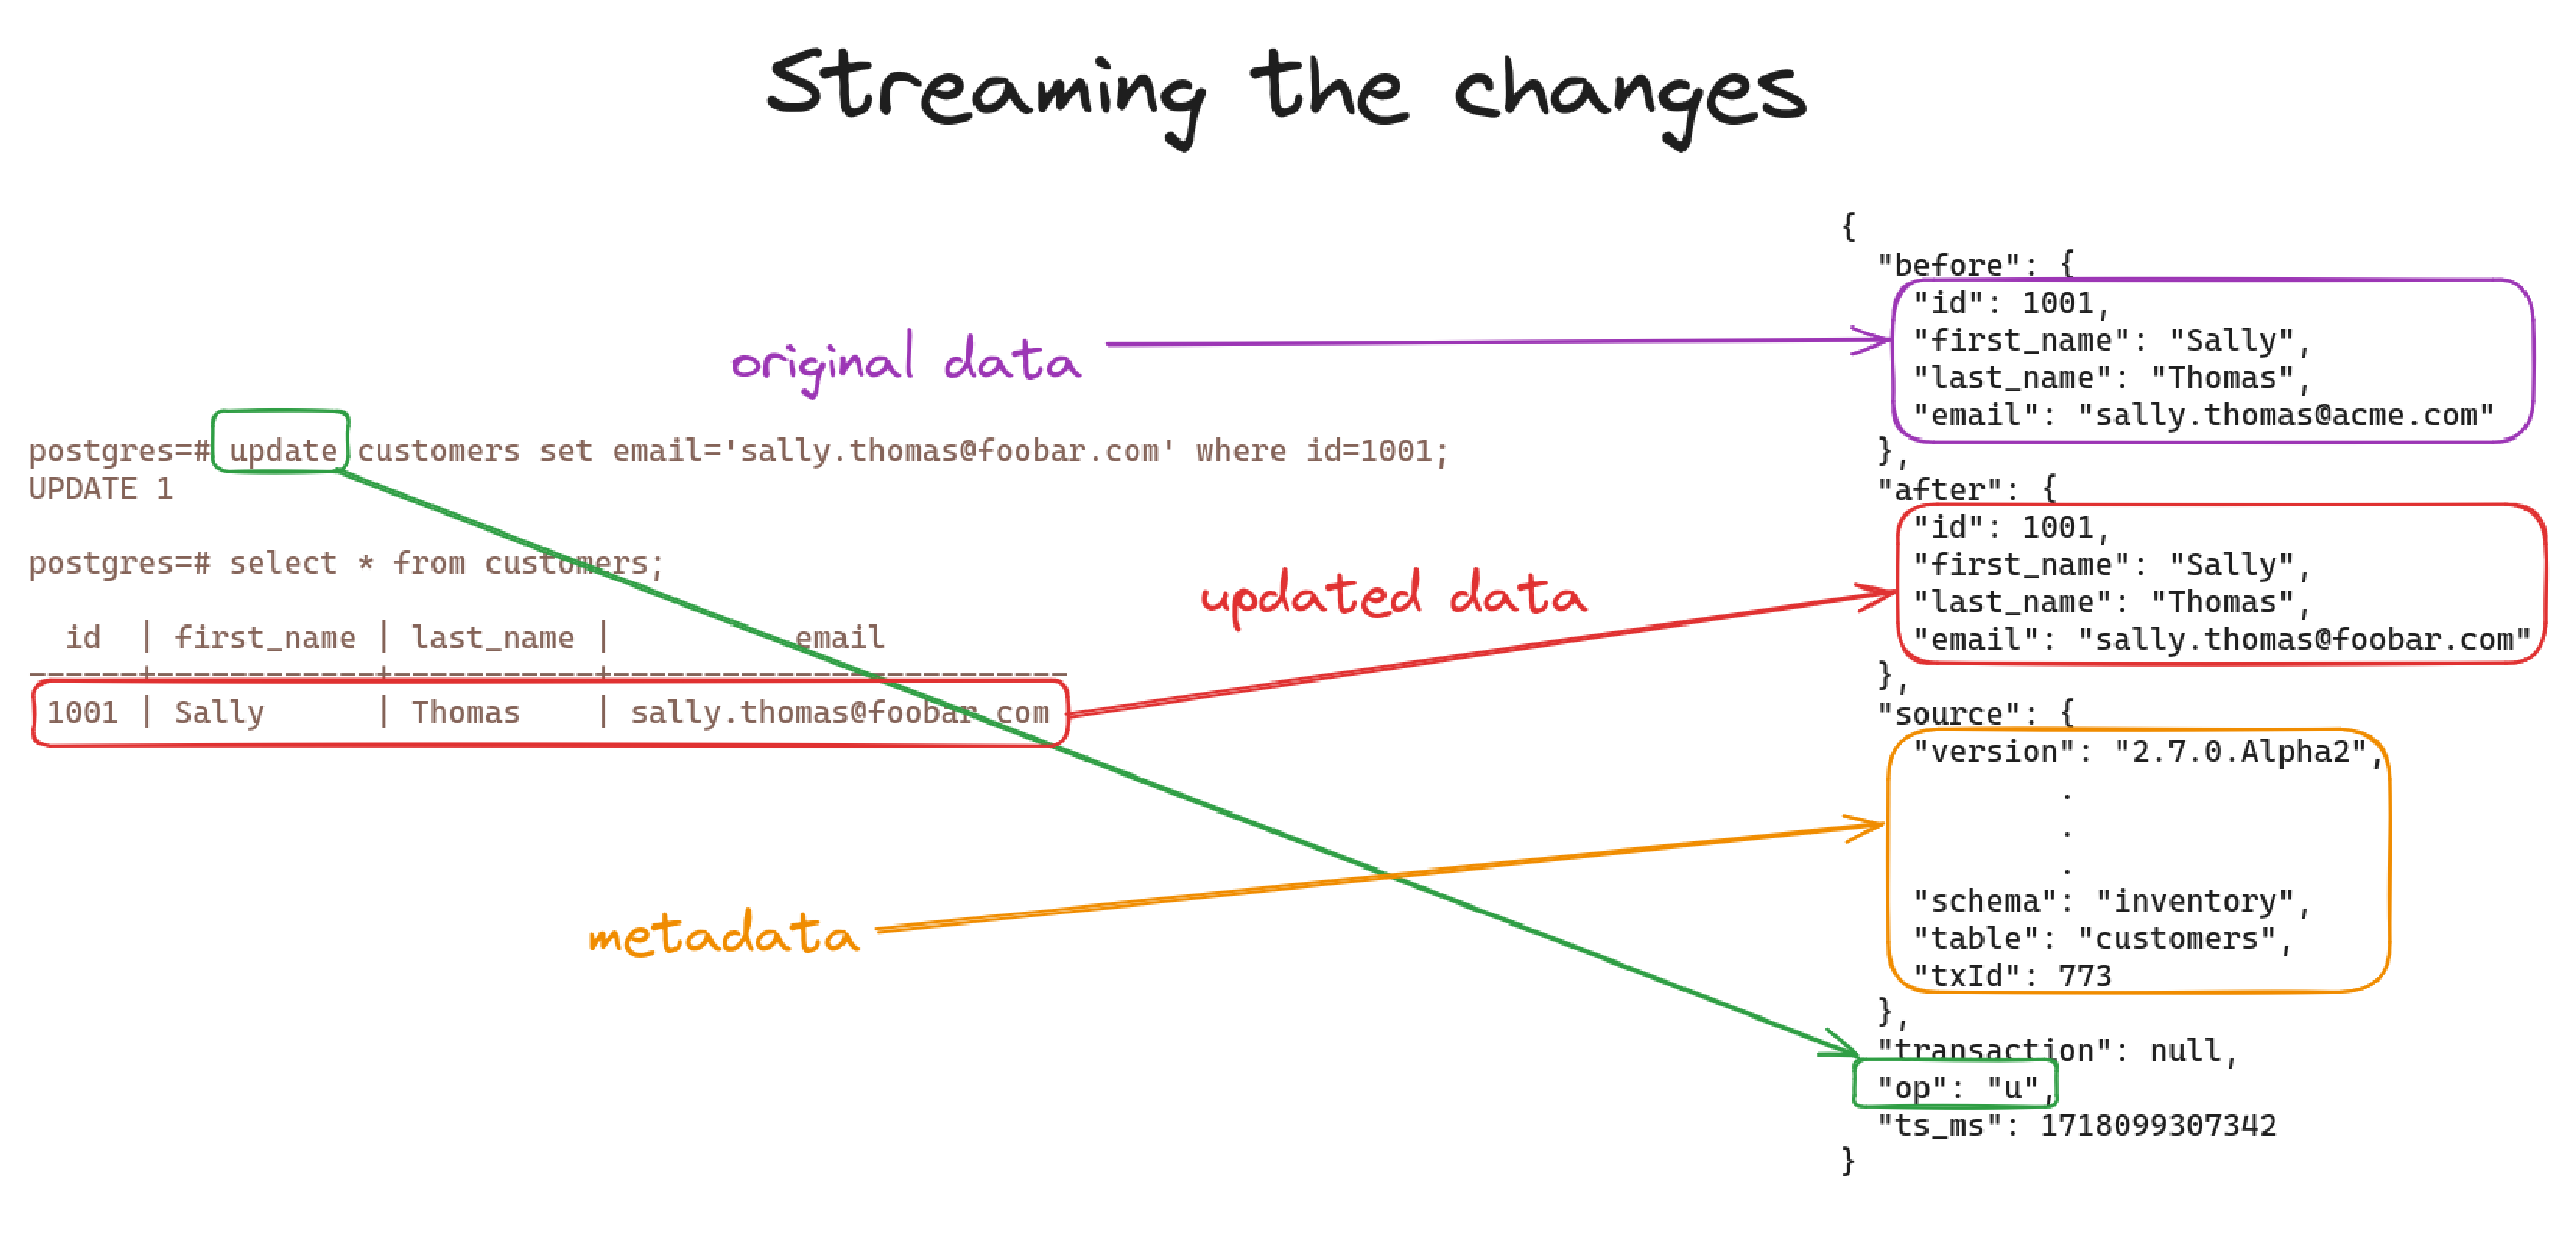
\includegraphics[height=5.5cm]{./img/update_data.eps}
    \end{figure}
\end{frame}

\begin{frame}
    \begin{figure}
        \centering
        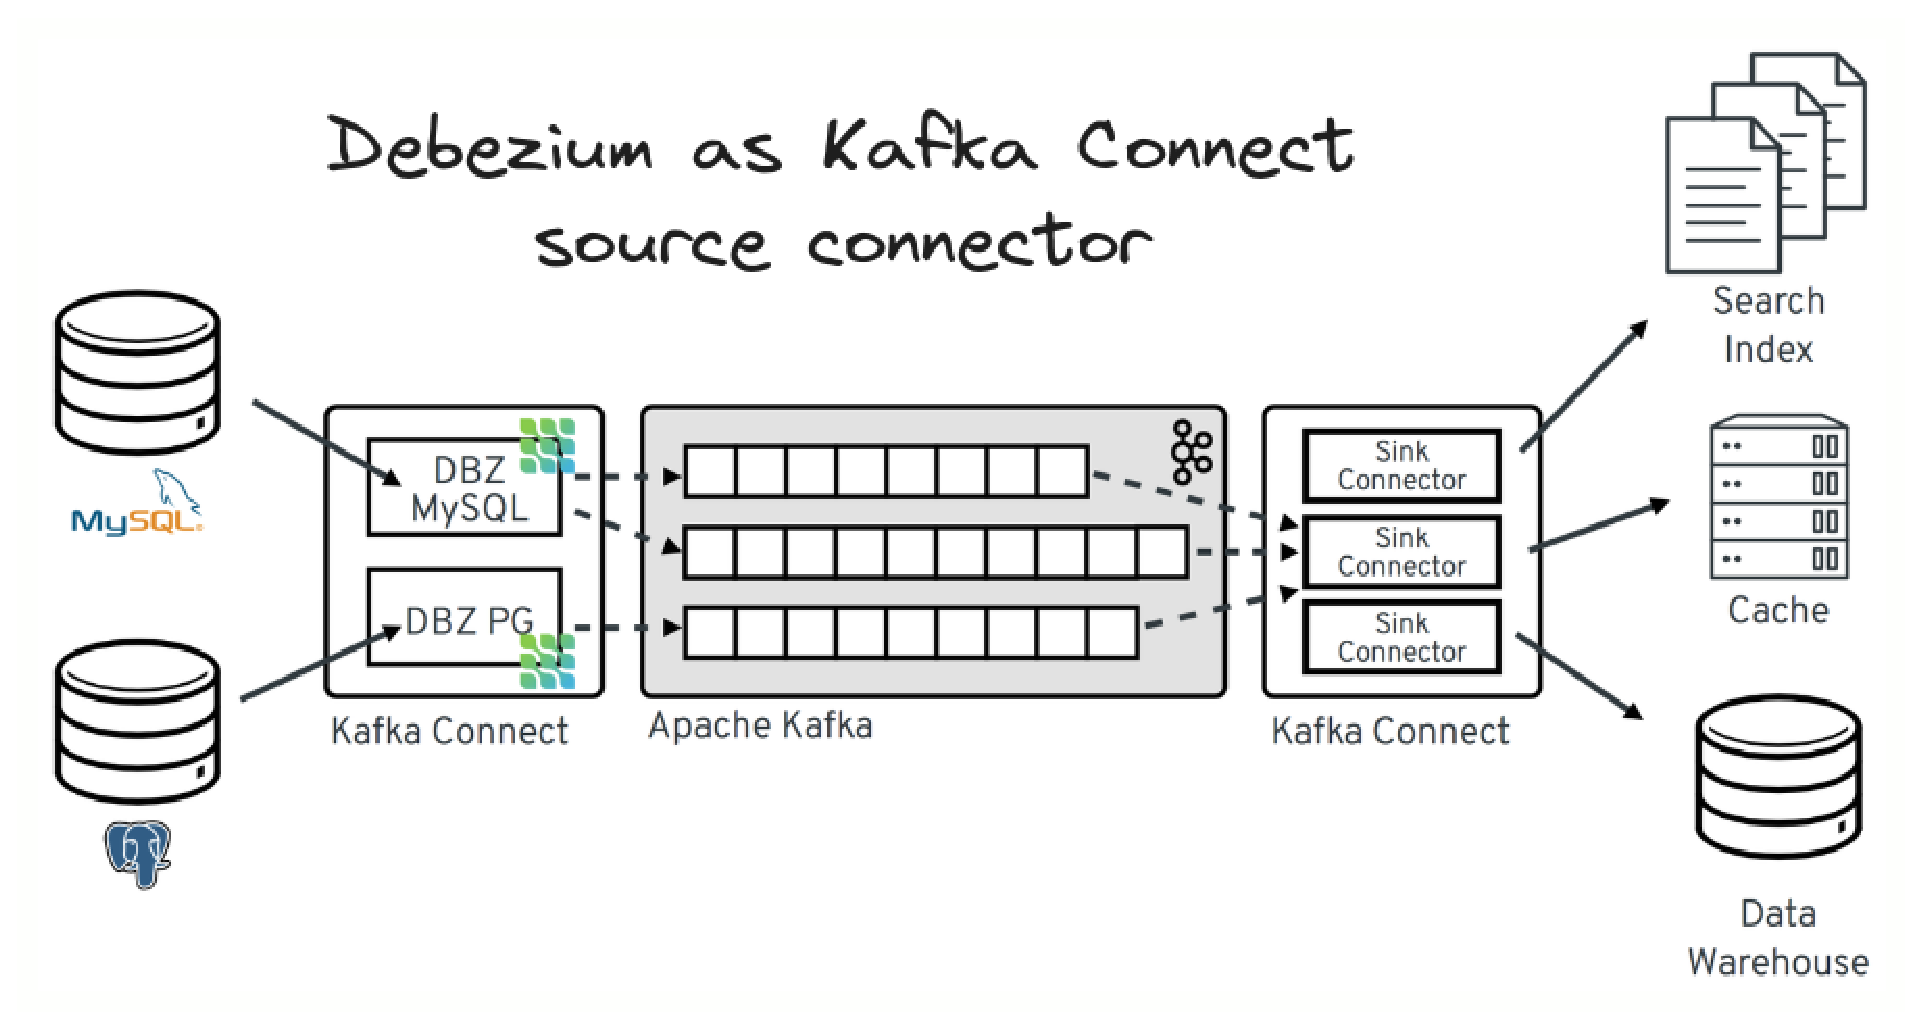
\includegraphics[height=6cm]{./img/debezium_kafka.eps}
    \end{figure}
\end{frame}    
    
\begin{frame}
    \begin{figure}
        \centering
        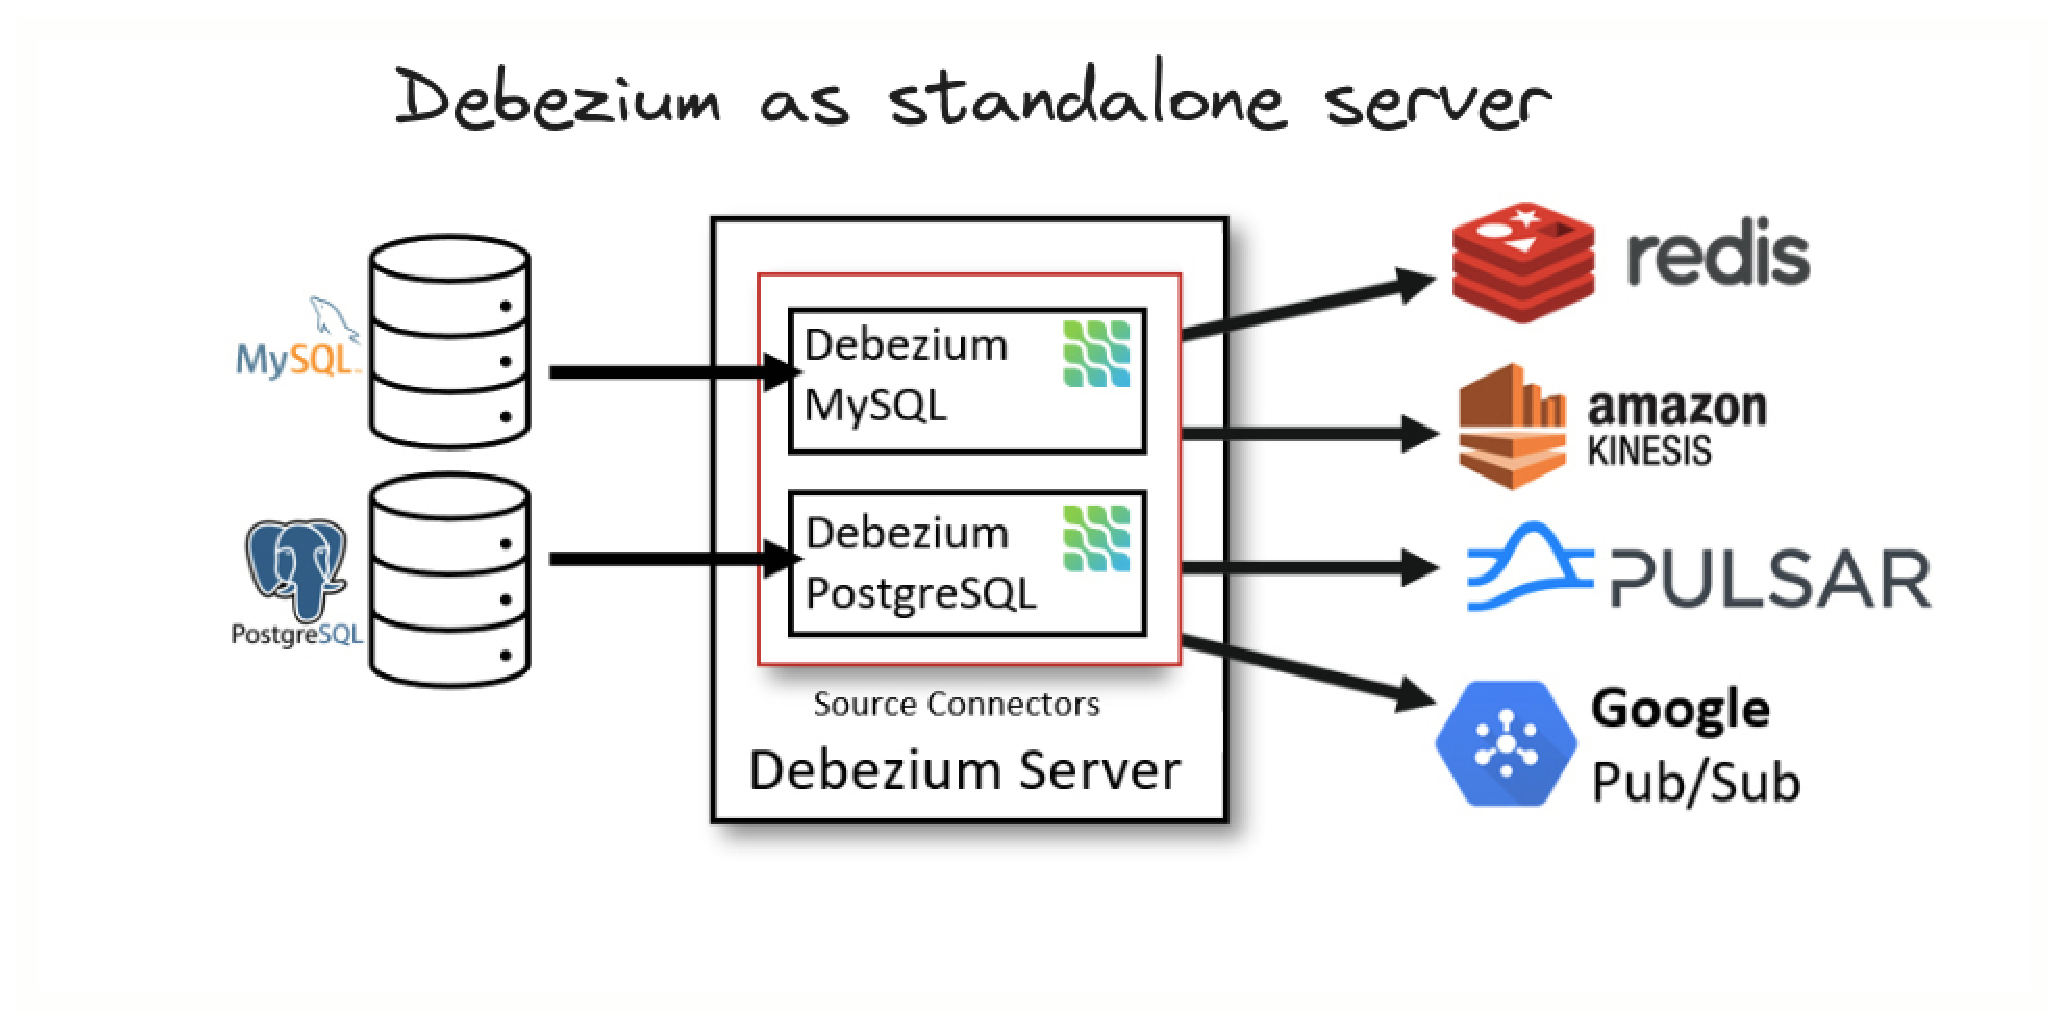
\includegraphics[height=6cm]{./img/debezium_server.eps}
    \end{figure}
\end{frame}    

\begin{frame}
    \begin{figure}
        \centering
        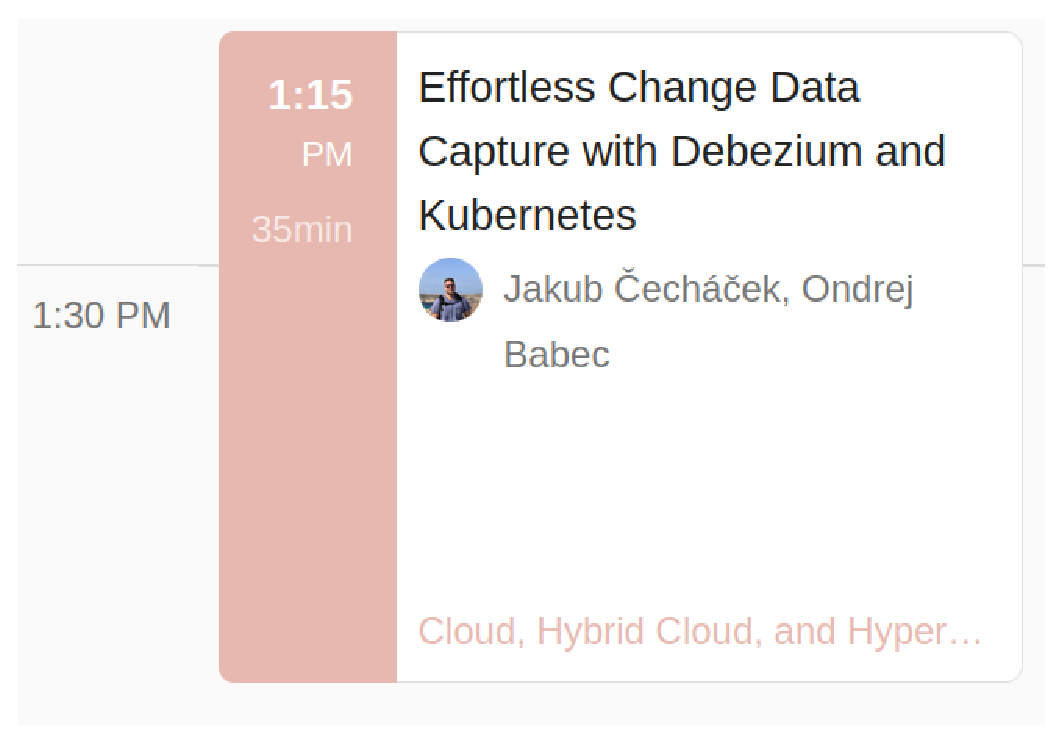
\includegraphics[height=8cm]{./img/dbz_k8s_talk.eps}
    \end{figure}
\end{frame}

\begin{frame}
    \vspace*{1cm}
    \centering
    \textbf{\huge{Back to the demo!}}
    
    \vspace*{0.5cm}
    
    \begin{figure}
        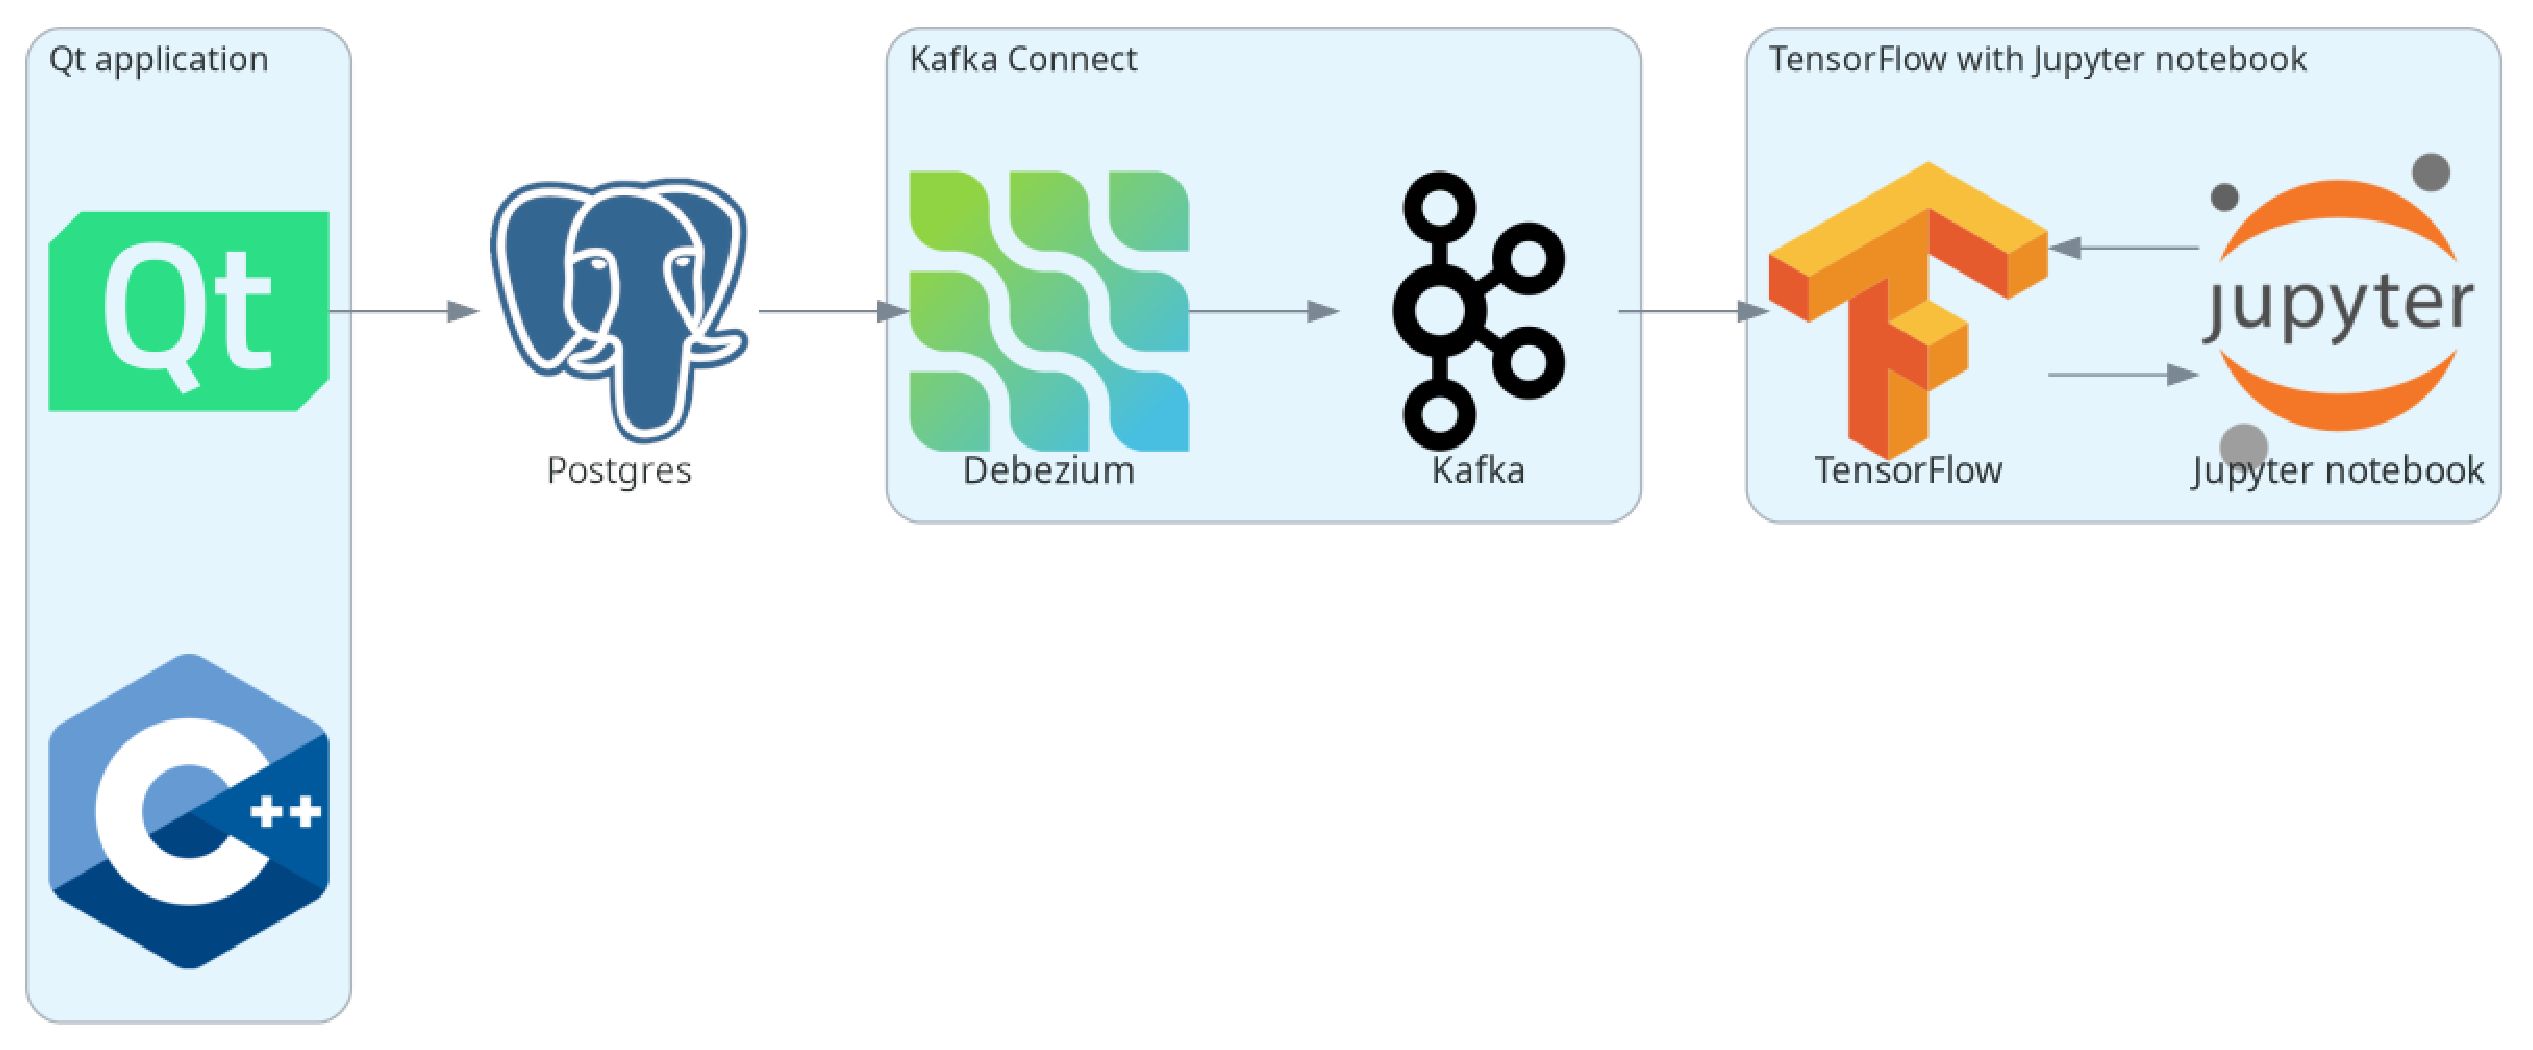
\includegraphics[height=4cm]{./img/qt_to_tf.eps}
    \end{figure}
    
    \vspace*{0.5cm}
    
    For more details see
    \begin{itemize}
        \color{blue}
        \item \href{https://debezium.io/blog/2023/05/02/tensorflow-mnist-classification}{Image classification with Debezium and TensorFlow blog post}
        \item \href{https://github.com/vjuranek/debezium-mnist-demo}{https://github.com/vjuranek/debezium-mnist-demo}
        \color{black}
    \end{itemize}
\end{frame}

\begin{frame}[fragile]
    \frametitle{Reading data from Kafka in TensorFlow}
    TensorFlow I/O provides \textcolor{blue}{\href{https://www.tensorflow.org/io/api_docs/python/tfio/experimental/streaming/KafkaGroupIODataset}{KafkaGroupIODataset}}:
    
    \vspace{0.5cm}
    
    \footnotesize
    \begin{python}
import tensorflow_io as tfio
    
# define Kafka data stream
test_ds = tfio.experimental.streaming.KafkaGroupIODataset(
    topics=[KAFKA_TEST_TOPIC],
    group_id=KAFKA_CONSUMER_GROUP,
    servers=KAFKA_SERVERS,
    stream_timeout=KAFKA_STREAM_TIMEOUT,
    configuration=[
        "session.timeout.ms=10000",
        "max.poll.interval.ms=10000",
        "auto.offset.reset=earliest"
    ],
)
    \end{python}
\end{frame}

\begin{frame}[fragile]
    \frametitle{Possible issues}
    \textbf{Deserialization issue in TensorFlow:}
    \vspace{0.5cm}
   \begin{lstlisting}
 <tf.Tensor: shape=(64,), dtype=string, numpy=
 array([b'[B@418b353d', b'[B@6aa28a4c',
        b'[B@3a3f1c1', b'[B@36e4ff1f',
        b'[B@765b7f70', b'[B@67567aa3',
        b'[B@58bc3a3a', b'[B@c6bc0ec',
        b'[B@64b48bac', b'[B@360a5b76',
        b'[B@3006c930', b'[B@54b3e5ad',
        b'[B@155dd43d', b'[B@5e88d5b6',
        b'[B@7dcdf024', b'[B@6570bf4e',
       dtype=object)>,
   \end{lstlisting}
\end{frame}

\begin{frame}[fragile]
    \frametitle{Single message transform (SMT) to rescue}
    \begin{itemize}
      \item Transform inbound and/or outbound messages.
      \item Can be used also e.g. for filtering to save bandwidth on the early stage of the ML pipeline.
      \item Many SMTs available out-of-the-box.
      \item Very easy to write custom SMT.
    \end{itemize}

    \vspace{0.5cm}
    
    \begin{lstlisting}[style=java]
$@Override$
public R apply(R r) {
    final Struct value = (Struct) r.value();
    String key = value.getInt16(labelFieldName).toString();

    StringBuilder builder = new StringBuilder();
    for (byte pixel : value.getBytes(pixlesFieldName)) {
        builder.append(pixel & 0xFF).append(",");
    }
    return r.newRecord(r.topic(), r.kafkaPartition(),
        Schema.STRING_SCHEMA, key,
        Schema.STRING_SCHEMA,
        builder.toString(), r.timestamp());
} 
     \end{lstlisting}
\end{frame}

\begin{frame}[fragile]
    \frametitle{Debezium configuration}
    \footnotesize
    \begin{lstlisting}[language=json, mathescape=true]
{
  "name": "mnist-connector",
  "config": {
    "connector.class": "io.debezium.connector.postgresql.PostgresConnector",
    "tasks.max": "1",
    "database.hostname": "postgres",
    "database.port": "5432",
    "database.user": "postgres",
    "database.password": "postgres",
    "database.dbname" : "postgres",
    "topic.prefix": "tf",
    $\textcolor{magenta}{\textbf{"table.include.list": "public.mnist\_.*",}}$
    "key.converter": "org.apache.kafka.connect.storage.StringConverter",
    "value.converter": "org.apache.kafka.connect.storage.StringConverter",
    $\textcolor{magenta}{\textbf{"transforms": "unwrap, mnist",}}$
    "transforms.unwrap.type": "io.debezium.transforms.ExtractNewRecordState",
    $\textcolor{magenta}{\textbf{"transforms.mnist.type": "io.debezium.transforms.MnistToCsv"}}$
  }
} 
     \end{lstlisting}
\end{frame}

\begin{frame}[fragile]
    \frametitle{Reading data in TensorFlow}
    \vspace{-0.2cm}
    \footnotesize
    \begin{python}
# define function for decoding Kafka records
def decode_kafka_stream_record(message, key):
    img_int = tf.io.decode_csv(message, [[0.0] for i in range(NUM_COLUMNS)])
    img_norm = tf.cast(img_int, tf.float32) / 255.
    label_int = tf.strings.to_number(key, out_type=tf.dtypes.int32)
    return (img_norm, label_int)
# define Kafka data stream
test_ds = tfio.experimental.streaming.KafkaGroupIODataset(
    topics=[KAFKA_TEST_TOPIC],
    group_id=KAFKA_CONSUMER_GROUP,
    servers=KAFKA_SERVERS,
    stream_timeout=KAFKA_STREAM_TIMEOUT,
    configuration=[
        "session.timeout.ms=10000",
        "max.poll.interval.ms=10000",
        "auto.offset.reset=earliest"
    ],
)
# read batches of Kafka records
test_ds = test_ds.map(decode_kafka_stream_record)
test_ds = test_ds.batch(BATCH_SIZE)
# make predictions on the data samples
model.evaluate(test_ds)
    \end{python}
\end{frame}

\begin{frame}
    \frametitle{Flink and Spark}
    \begin{figure}
        \hspace*{-1.1cm}
        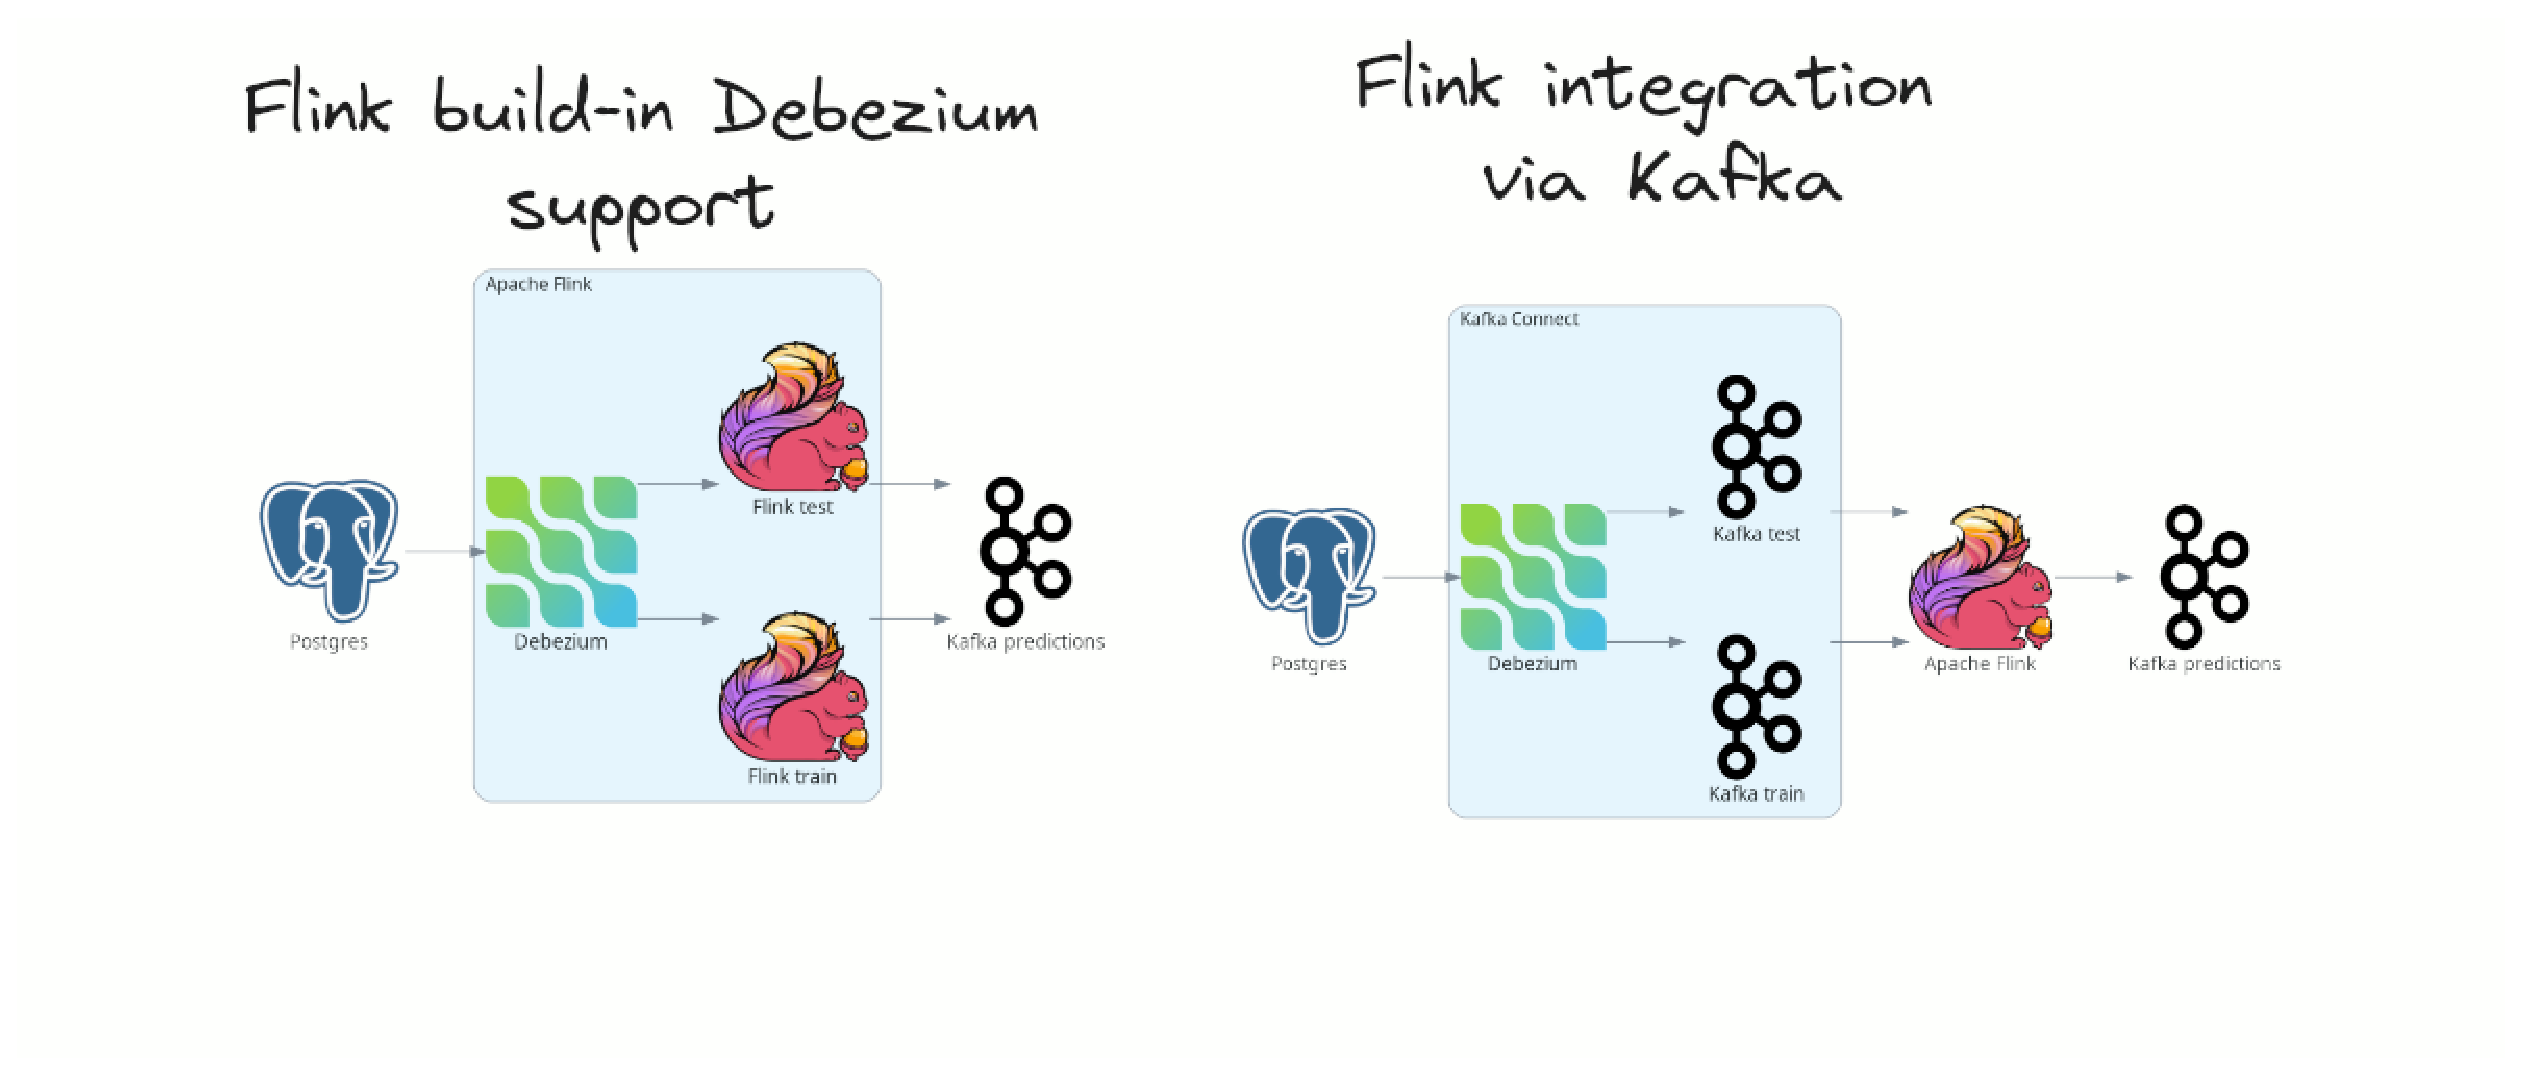
\includegraphics[height=6cm]{./img/debezium_flink.eps}
    \end{figure}
    
    \vspace{-1cm}
    Similar for Apache Spark.
    \vspace{0.5cm}
    
    For more details see
    \begin{itemize}
        \item  \footnotesize \color{blue}\url{https://debezium.io/blog/2023/09/23/flink-spark-online-learning}
        \item  \footnotesize \url{https://github.com/debezium/debezium-examples/tree/main/machine-learning/flink-spark-iris}\color{black}
    \end{itemize}
\end{frame}

\begin{frame}
    \frametitle{Feature stores}
    \begin{itemize}
        \item A centralized repository of features.
        \item Consistency across training and inference.
        \item Collaboration and reuseability.
        \item Precomping features.
        \item Monitoring for feature drift.
        \item Versioning.
        \item Integration with other MLOps tools, unified access to the features.
    \end{itemize}

     \begin{figure}
        \centering
        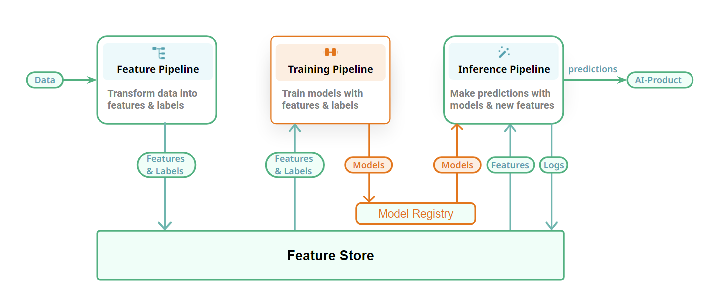
\includegraphics[height=4cm]{./img/featurestore.eps}
        \caption{\tiny{Source: \url{https://www.hopsworks.ai/dictionary/feature-store}}}
    \end{figure}
\end{frame}

\begin{frame}
    \begin{figure}
        \centering
        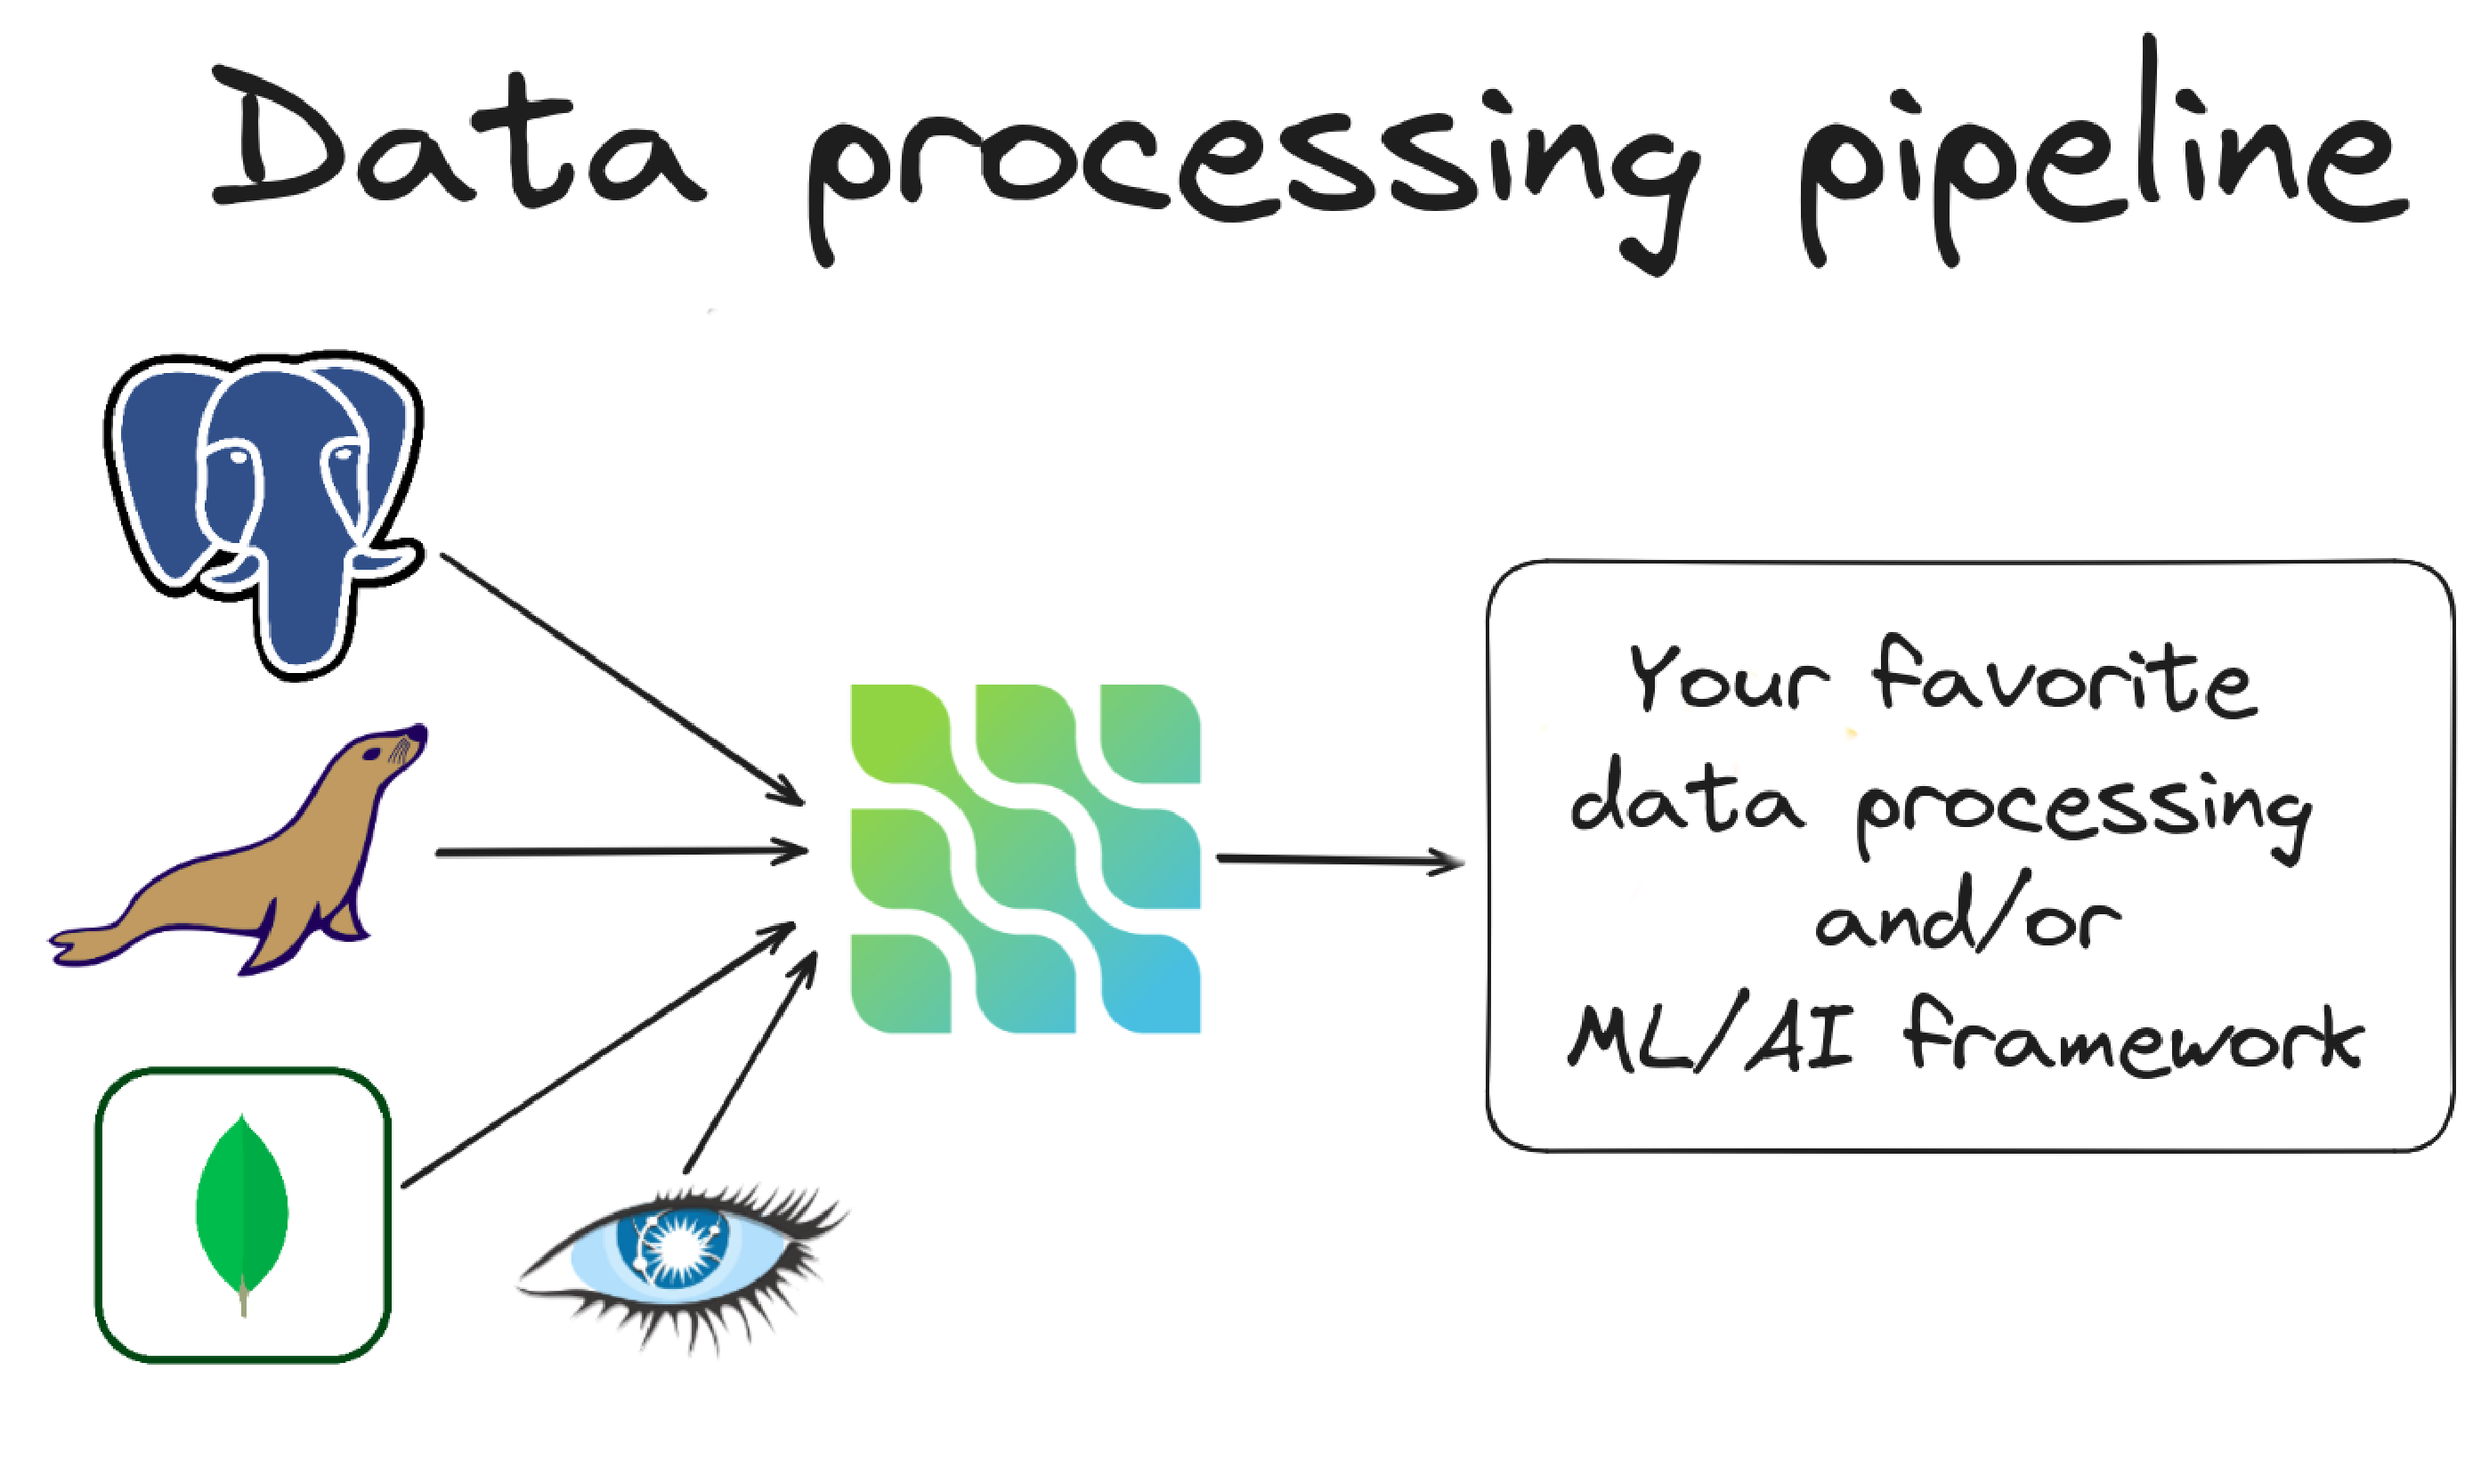
\includegraphics[height=6cm]{./img/dbs_to_ml.eps}
    \end{figure}
\end{frame}

\begin{frame}
    \centering
    \textbf{\Huge{Thank you!}}
    
    \vspace{1cm}
    
    \begin{figure}
        \centering
        
\includegraphics[height=1.5cm]{./img/debezium.eps}
    \end{figure}
    
    \vspace{0.5cm}
    
    \centering
    \color{blue}
    \url{https://debezium.io}\\
    \url{https://github.com/debezium}\\
    \url{https://debezium.zulipchat.com}\\
    \url{https://groups.google.com/g/debezium}\\
    \color{black}
\end{frame}

%%%%%%%%%%%%%%%%%%%%%%%%%%%%%%%%%%%%%%%%%%%%%%%%%%%%%%%%%%%%%%%%%%%%%%%%%%%%%%%%%%%%%%%%%%%%%%%%%
%%% BACKUP
%%%%%%%%%%%%%%%%%%%%%%%%%%%%%%%%%%%%%%%%%%%%%%%%%%%%%%%%%%%%%%%%%%%%%%%%%%%%%%%%%%%%%%%%%%%%%%%%%

% \begin{frame}
%     \centering
%     \huge{\textbf{Backup slides}}
% \end{frame}

\end{document}
